\newpage
\appendix
\onecolumn

\begin{figure}[t]
    \centering
    \begin{subfigure}[b]{0.32\textwidth}
        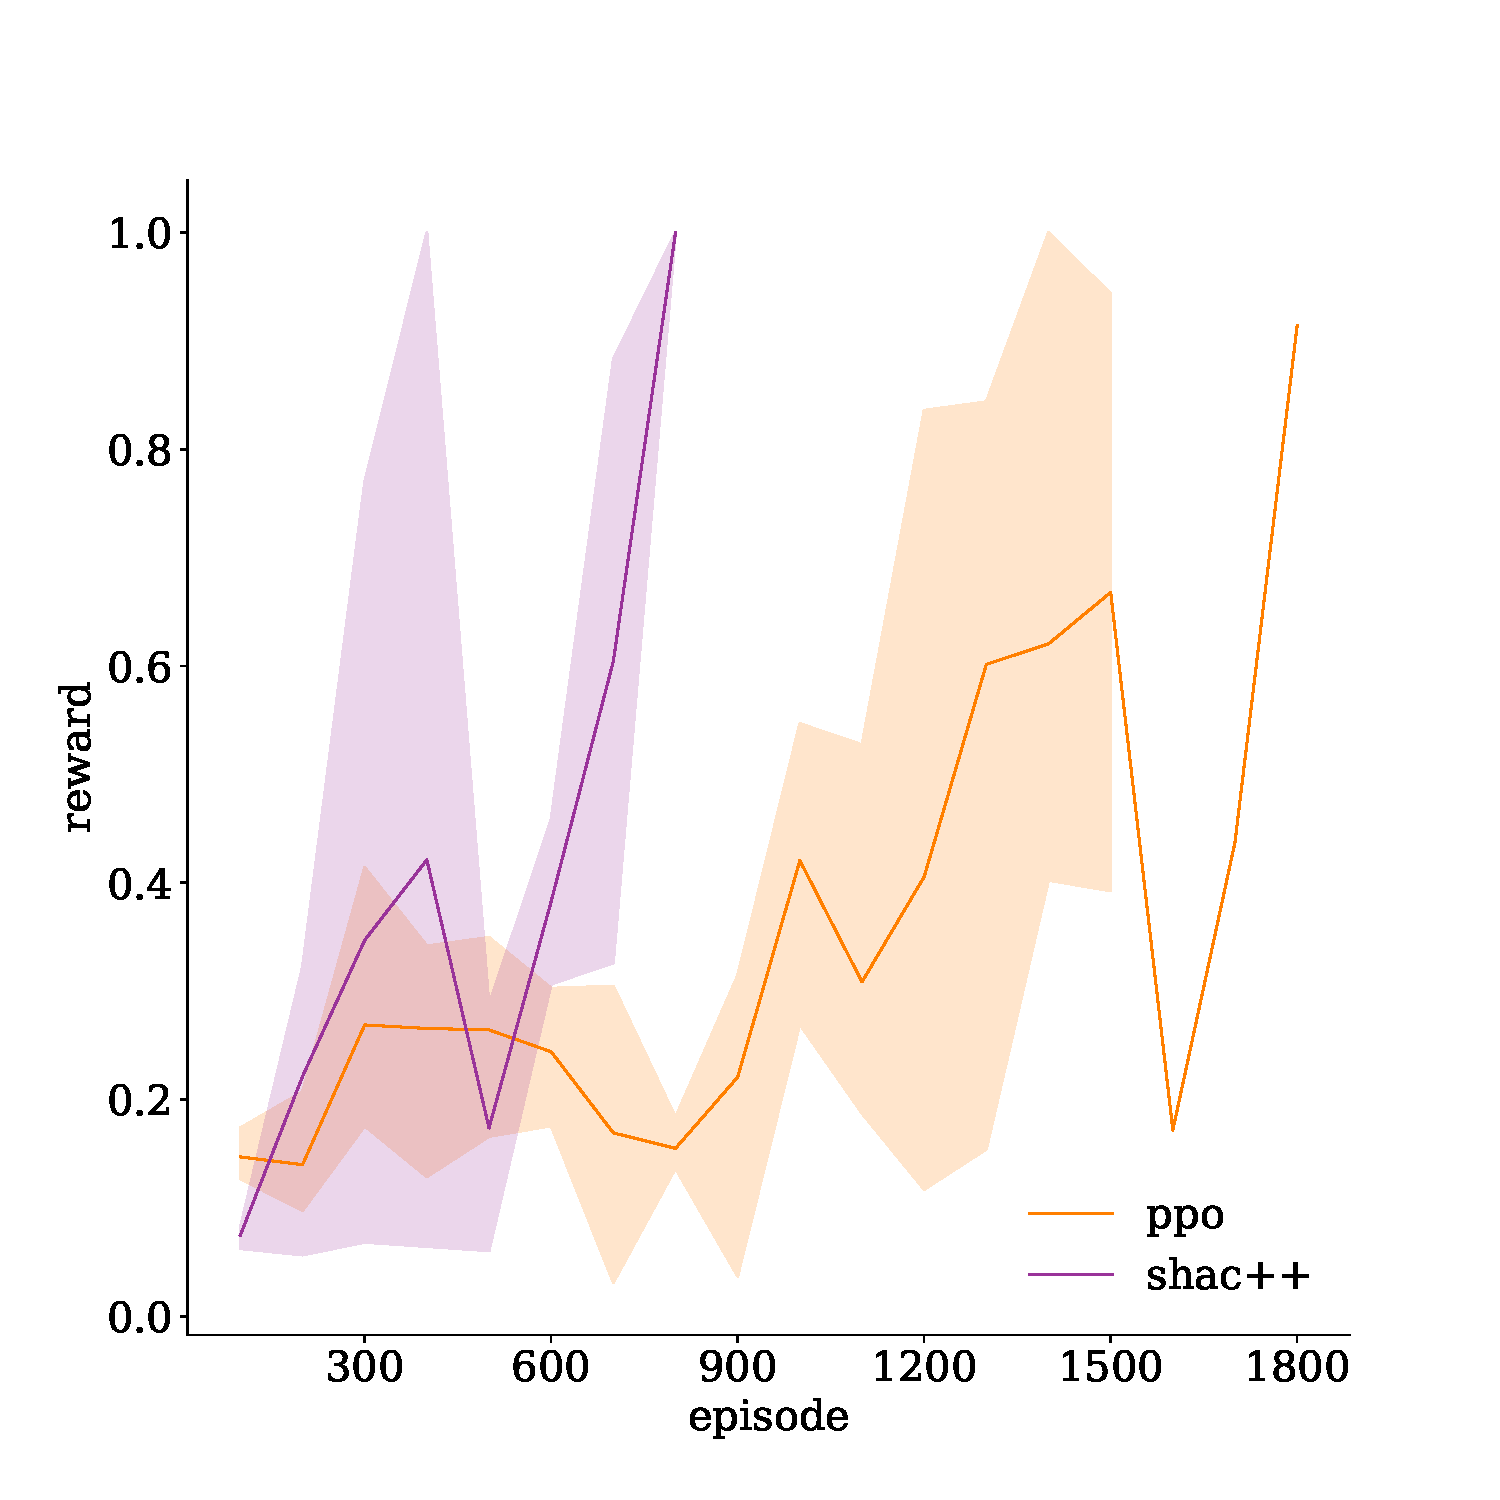
\includegraphics[width=\textwidth]{figs/dispersion-1-mlp.pdf}
        \caption{Dispersion, MLP, 1 agent}
        \label{apx:fig:dispersion-mlp-1}
    \end{subfigure}
    \begin{subfigure}[b]{0.32\textwidth}
        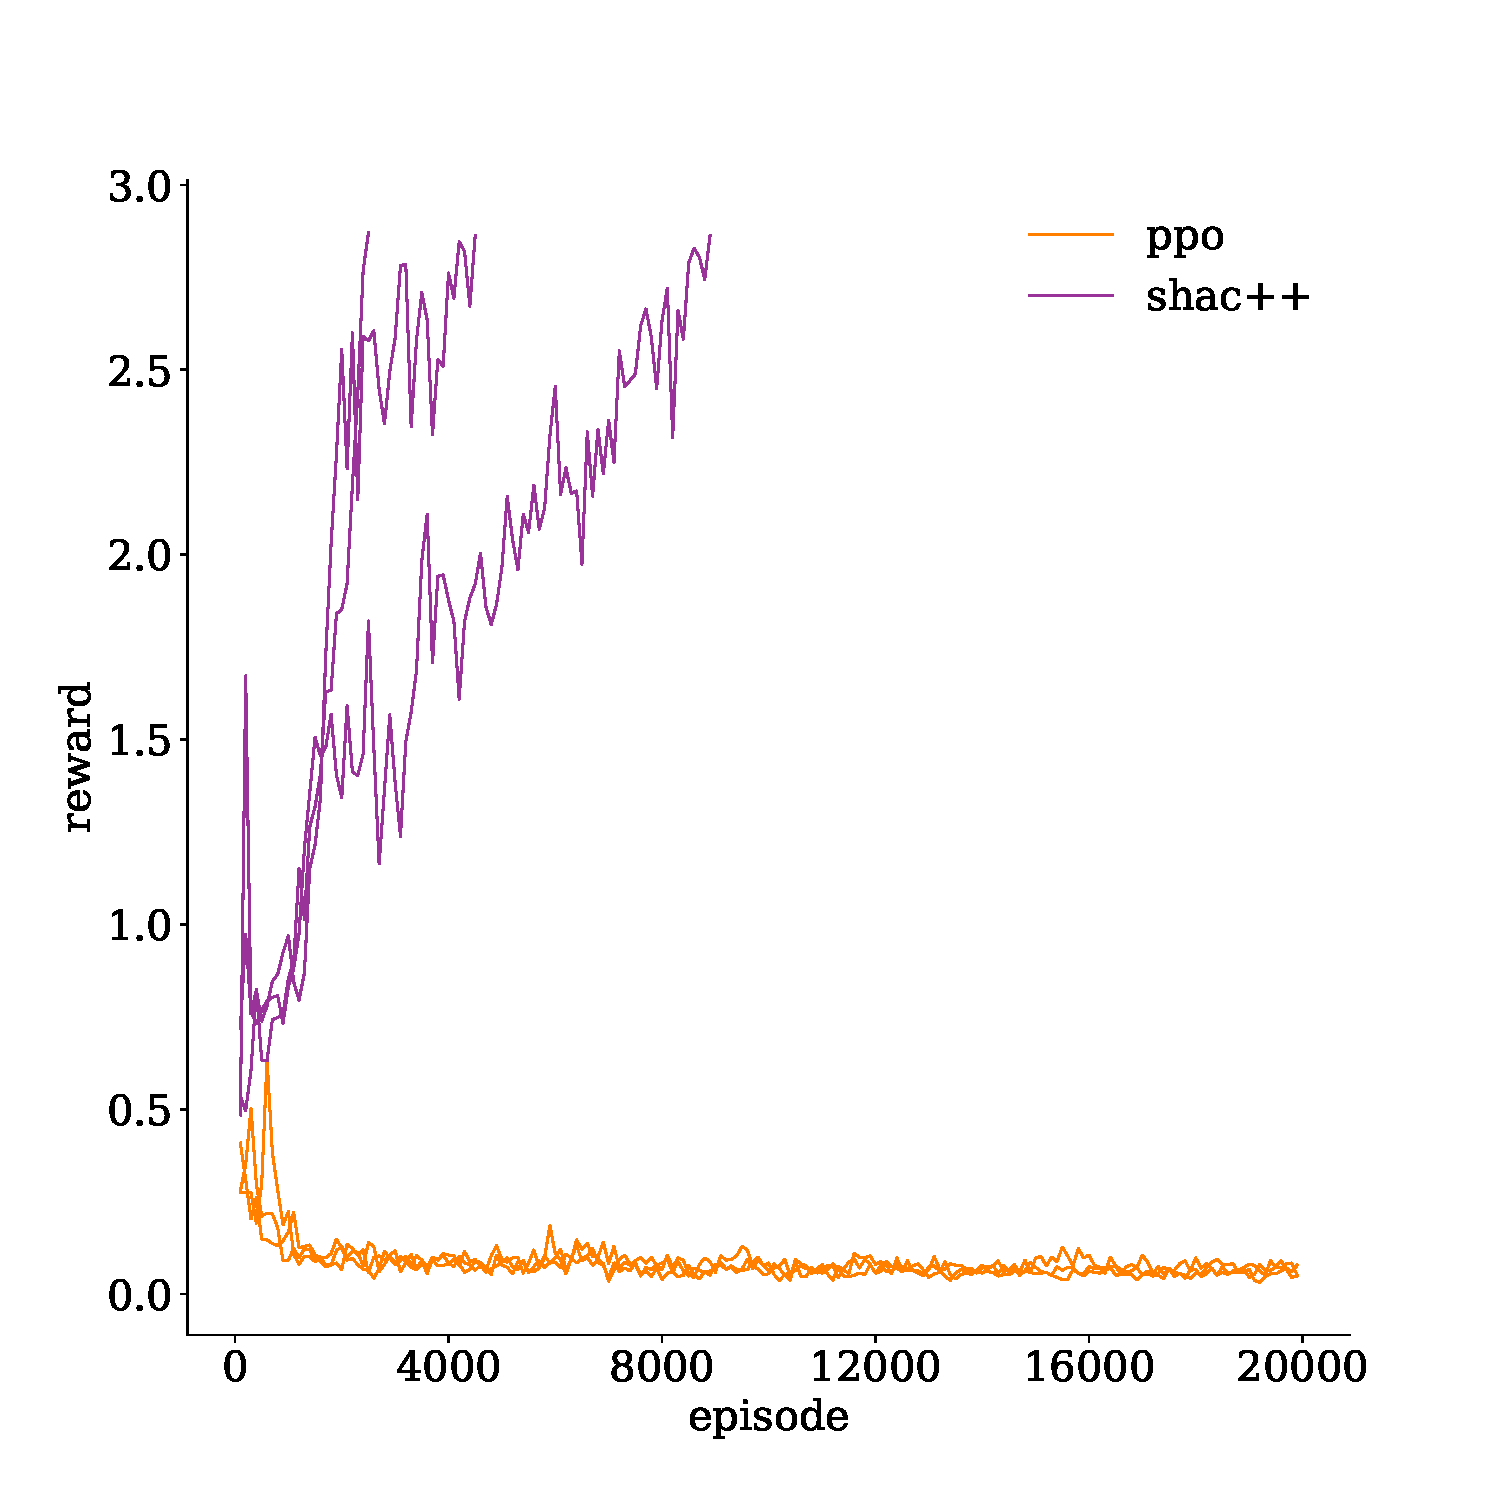
\includegraphics[width=\textwidth]{figs/dispersion-3-mlp.pdf}
        \caption{Dispersion, MLP, 3 agents}
        \label{apx:fig:dispersion-mlp-3}
    \end{subfigure}
    \begin{subfigure}[b]{0.32\textwidth}
        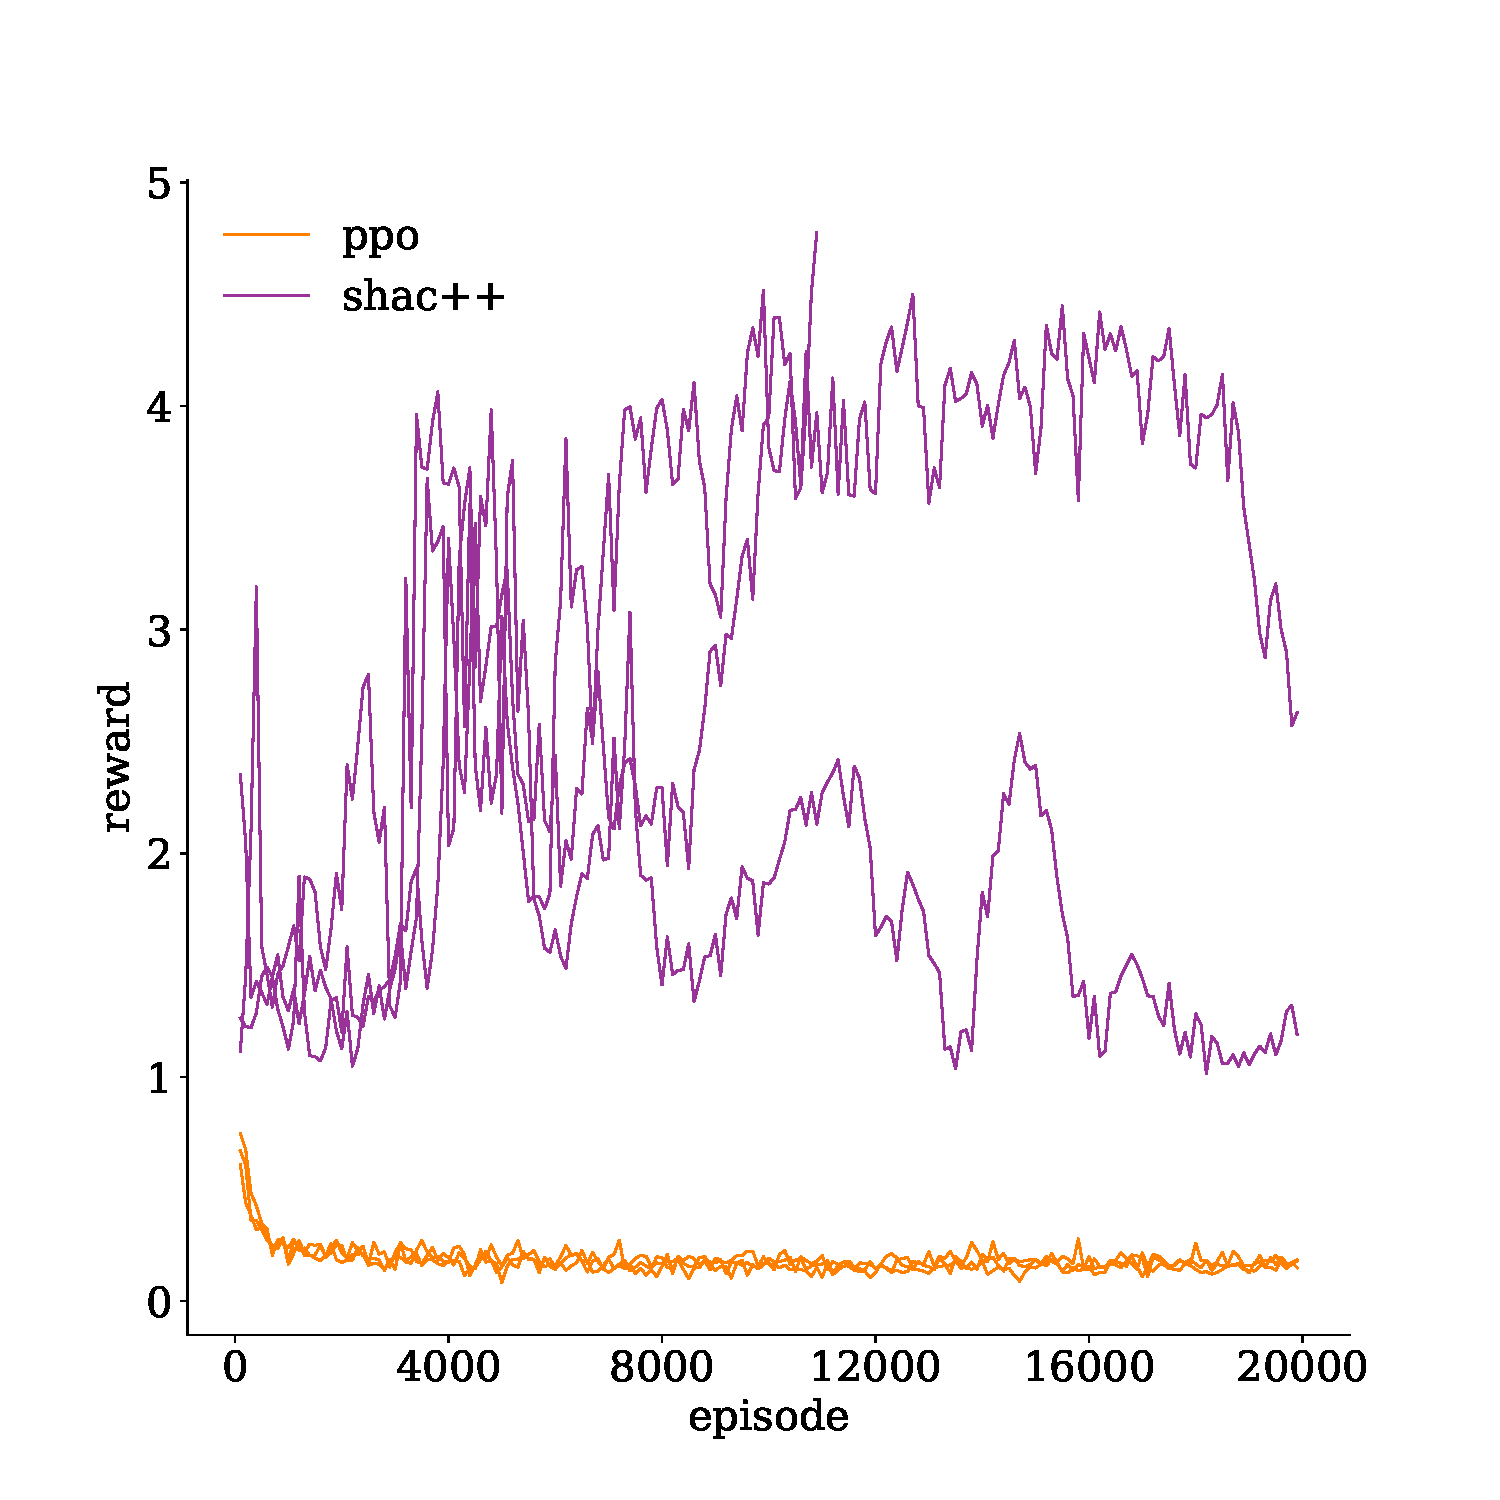
\includegraphics[width=\textwidth]{figs/dispersion-5-mlp.pdf}
        \caption{Dispersion, MLP, 5 agents}
        \label{apx:fig:dispersion-mlp-5}
    \end{subfigure}

    \begin{subfigure}[b]{0.32\textwidth}
        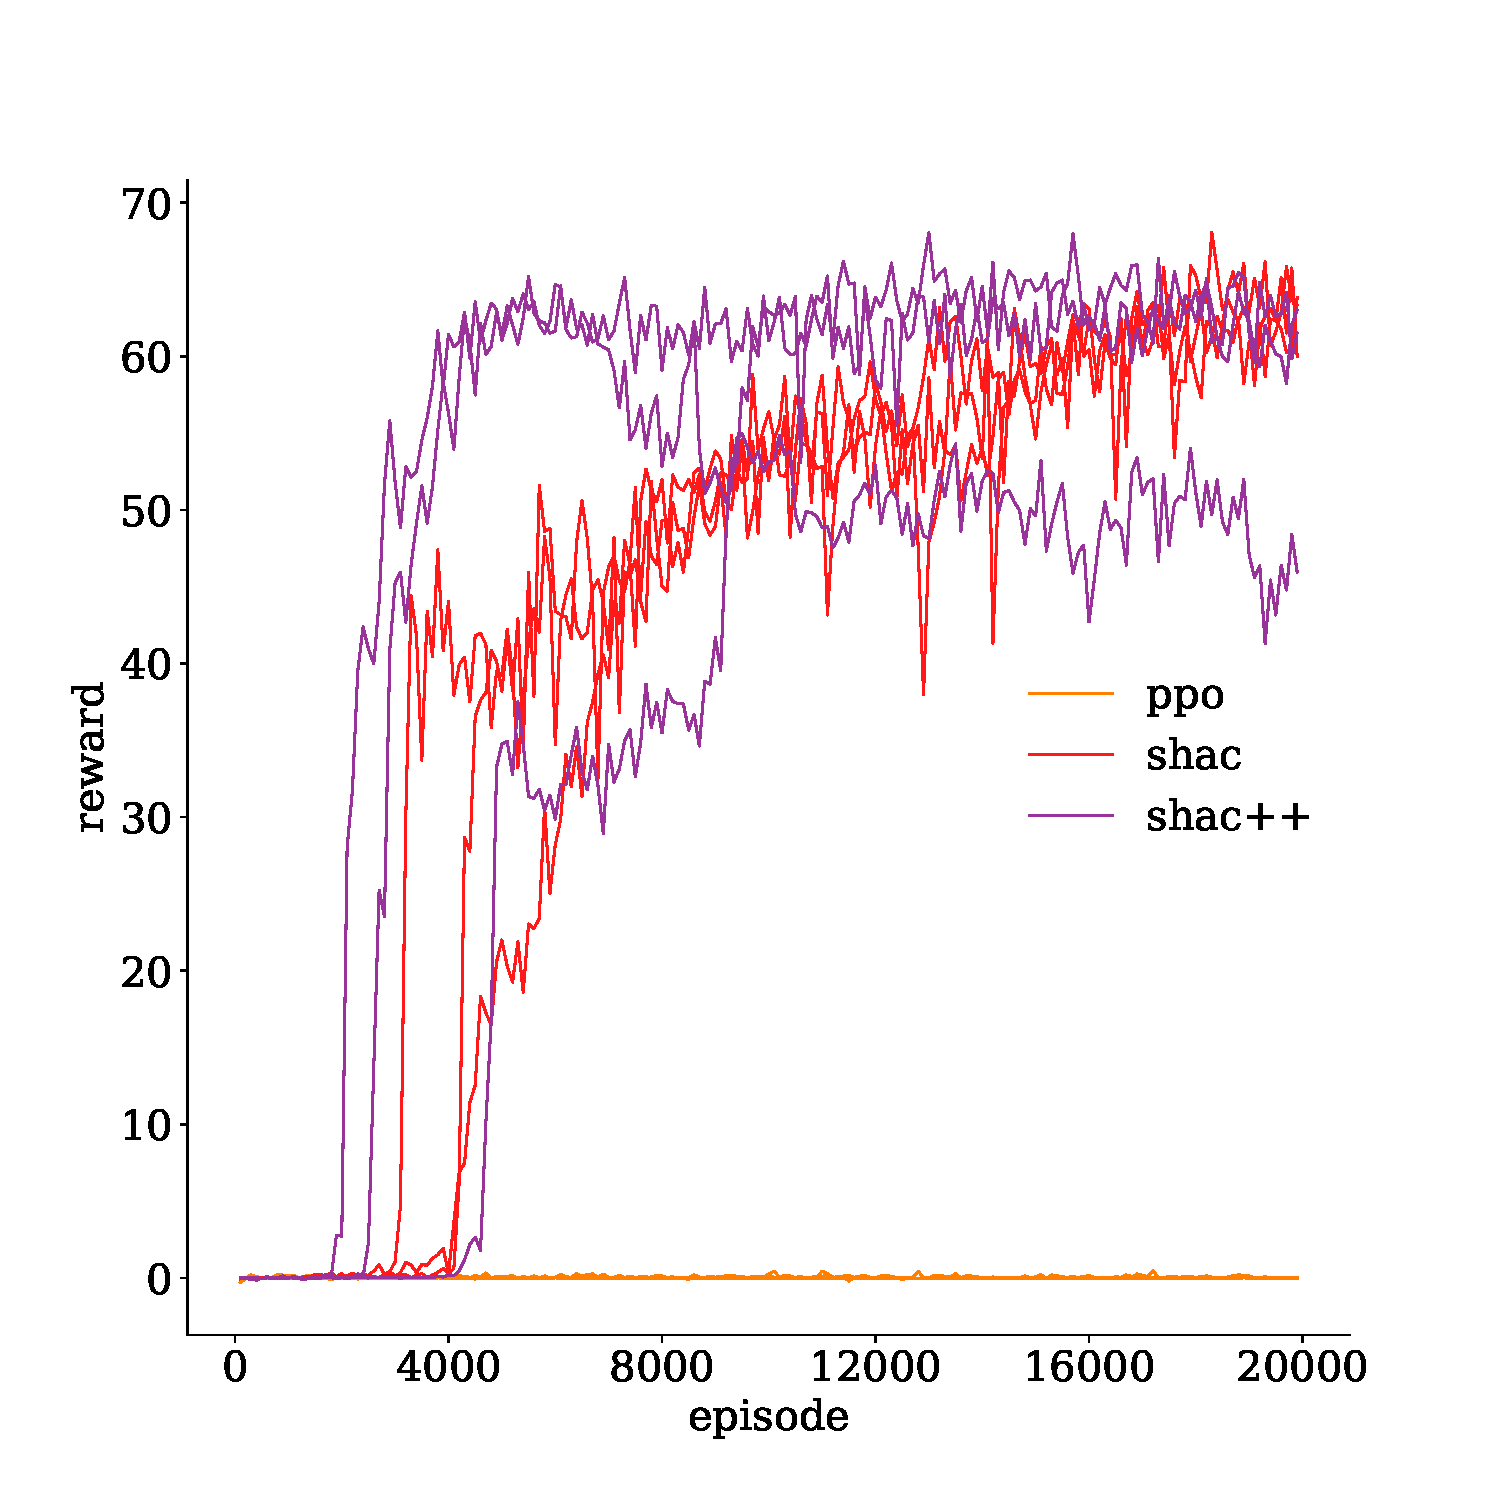
\includegraphics[width=\textwidth]{figs/transport-1-mlp.pdf}
        \caption{Transport, MLP, 1 agent}
        \label{apx:fig:transport-mlp-1}
    \end{subfigure}
    \begin{subfigure}[b]{0.32\textwidth}
        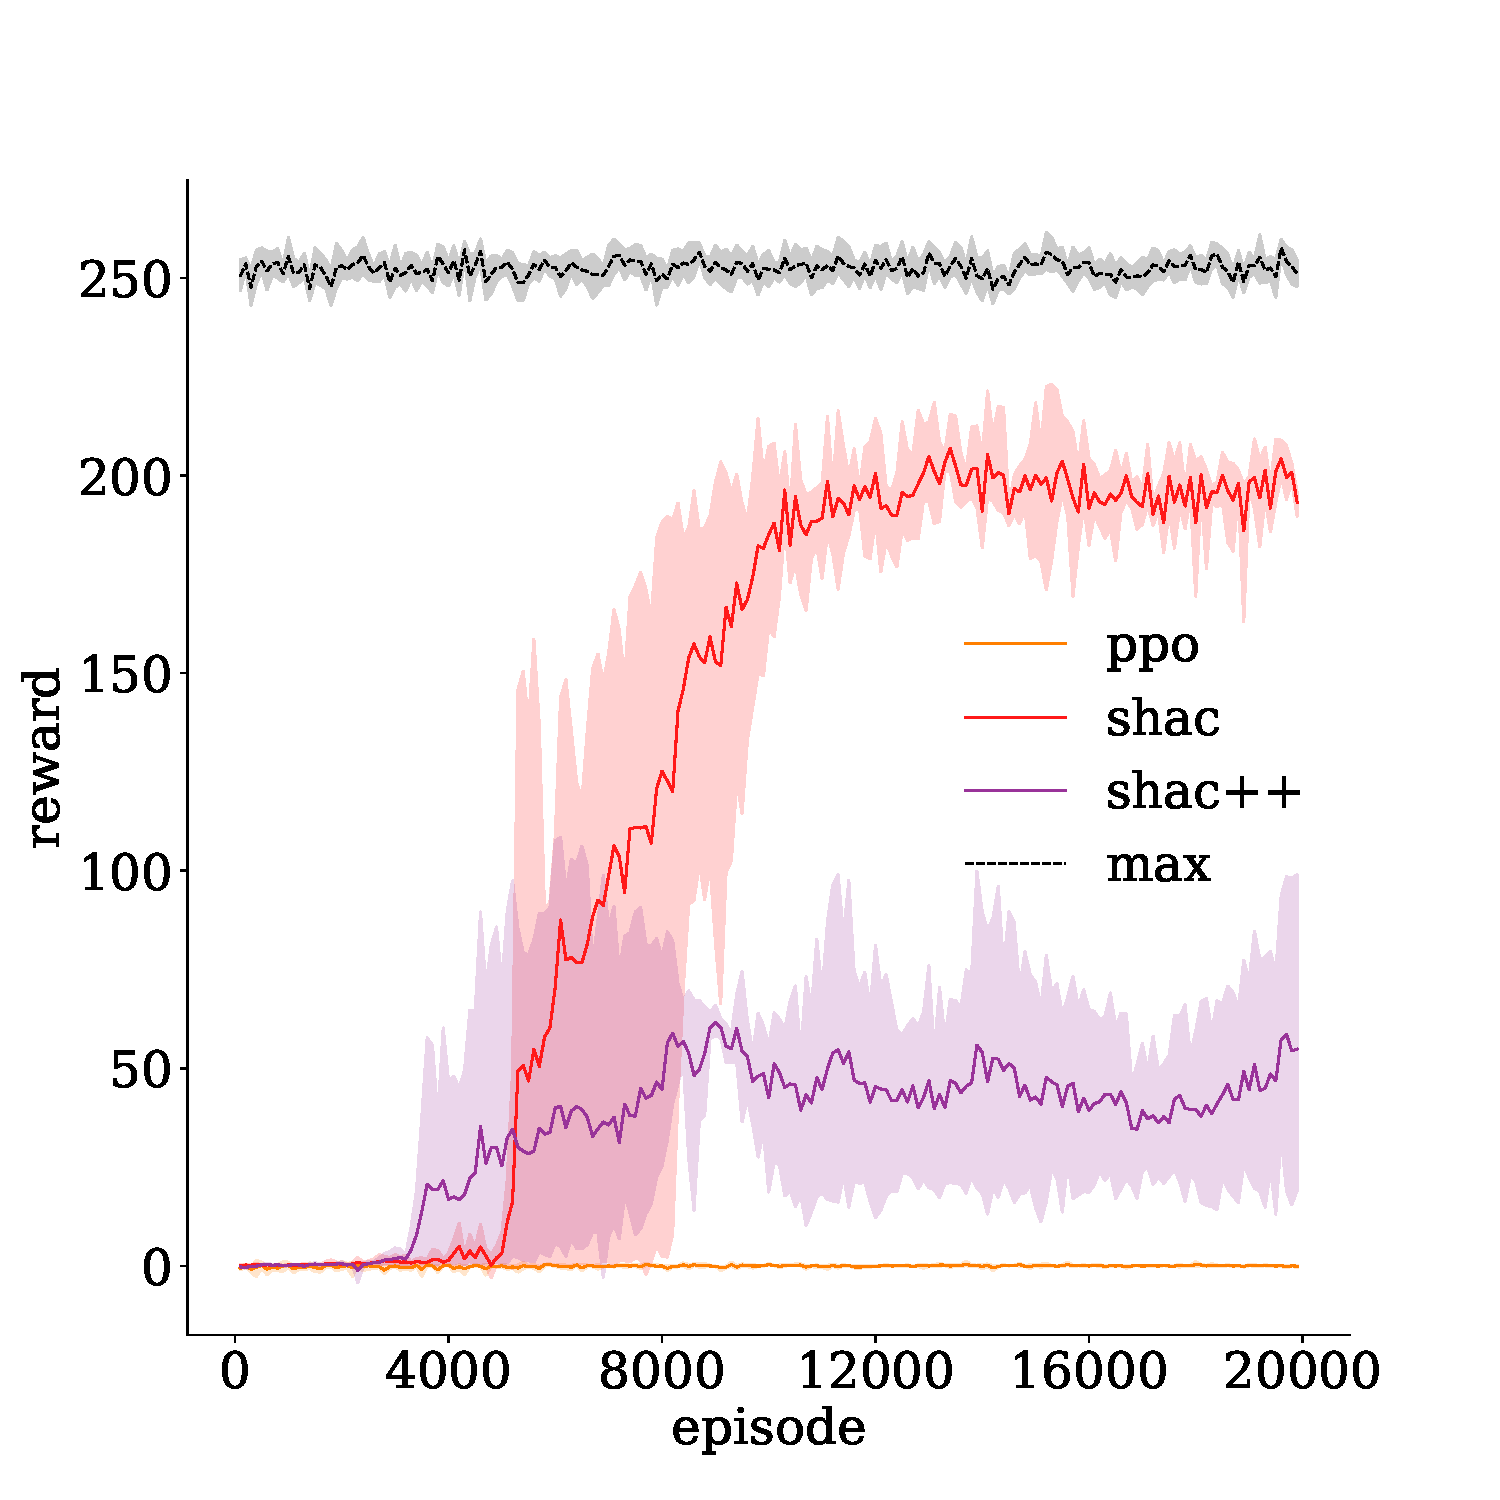
\includegraphics[width=\textwidth]{figs/transport-3-mlp.pdf}
        \caption{Transport, MLP, 3 agents}
        \label{apx:fig:transport-mlp-3}
    \end{subfigure}
    \begin{subfigure}[b]{0.32\textwidth}
        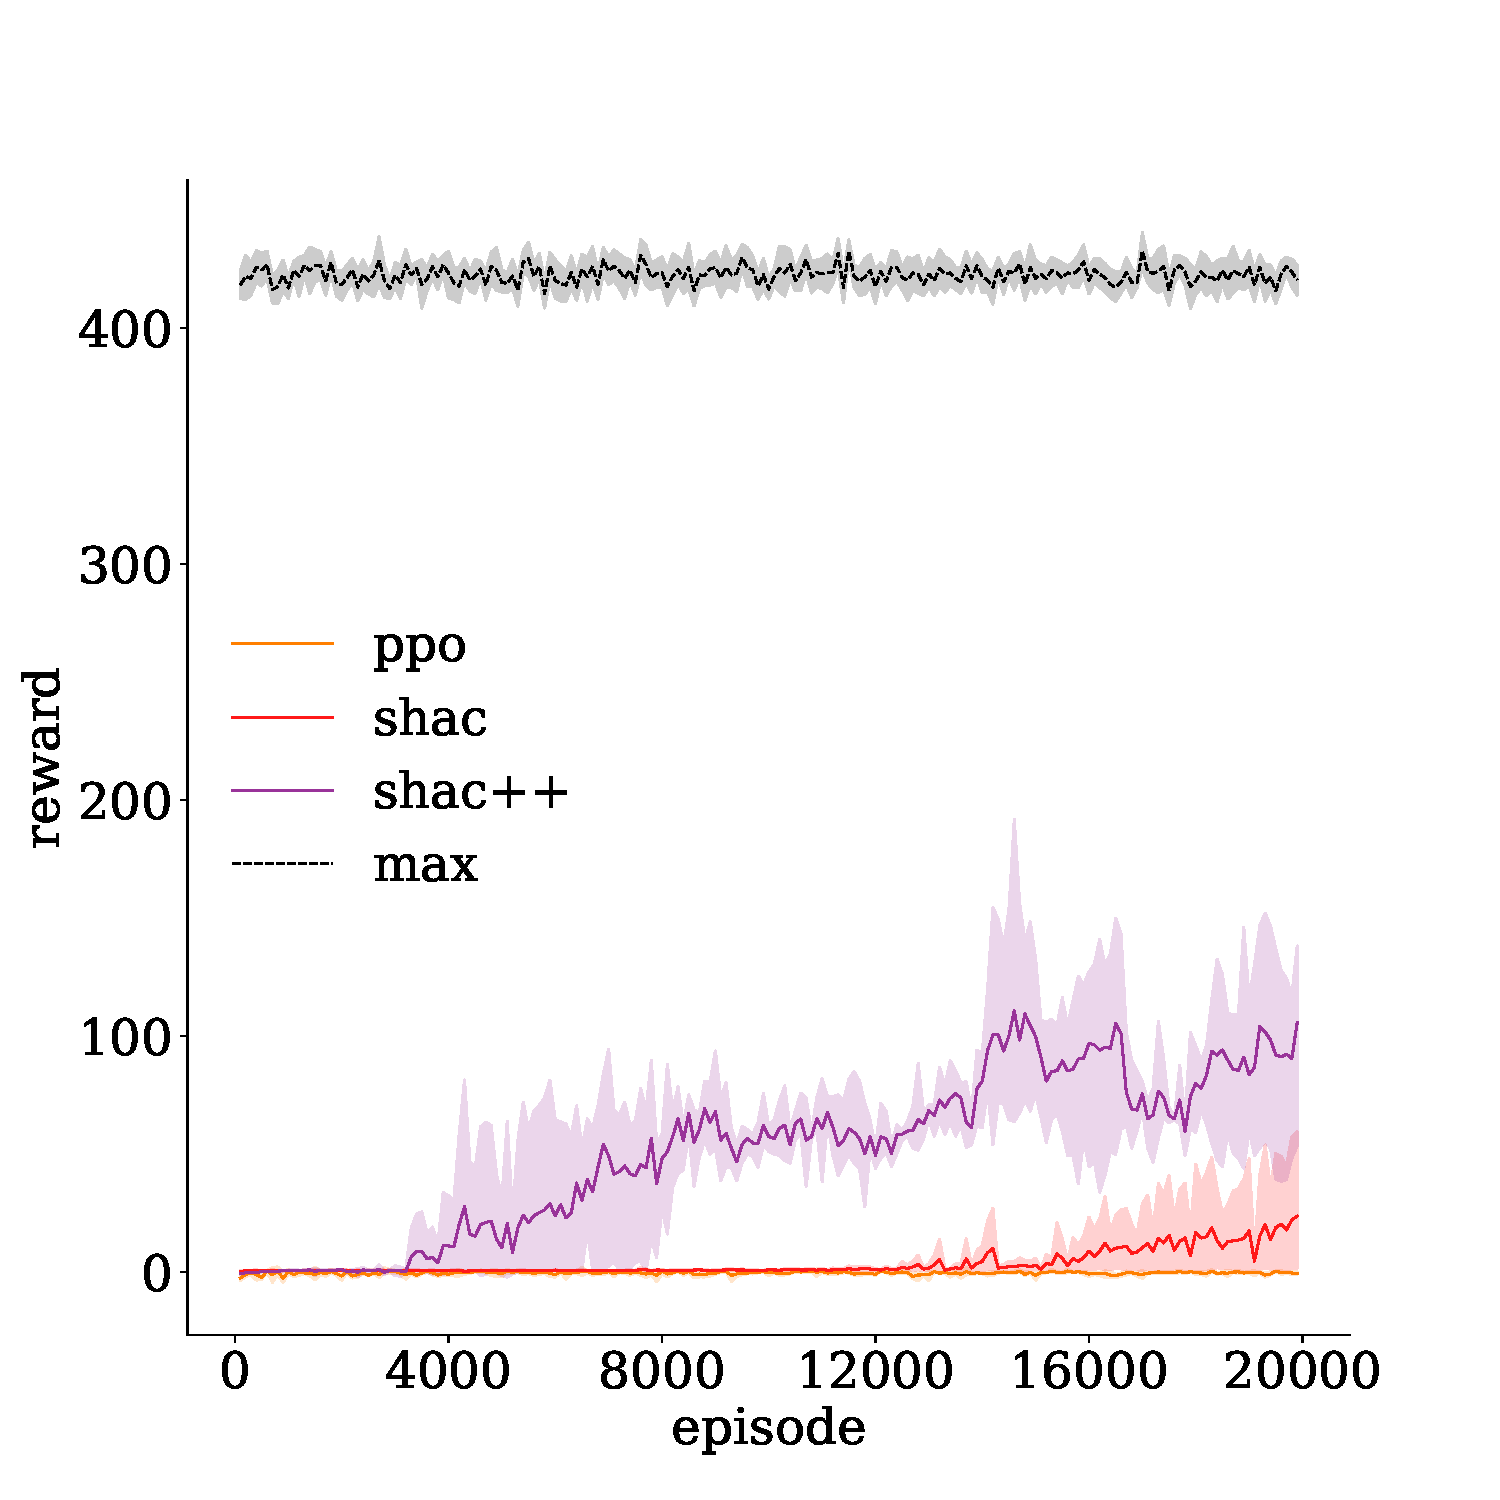
\includegraphics[width=\textwidth]{figs/transport-5-mlp.pdf}
        \caption{Transport, MLP, 5 agents}
        \label{apx:fig:transport-mlp-5}
    \end{subfigure}

    \begin{subfigure}[b]{0.32\textwidth}
        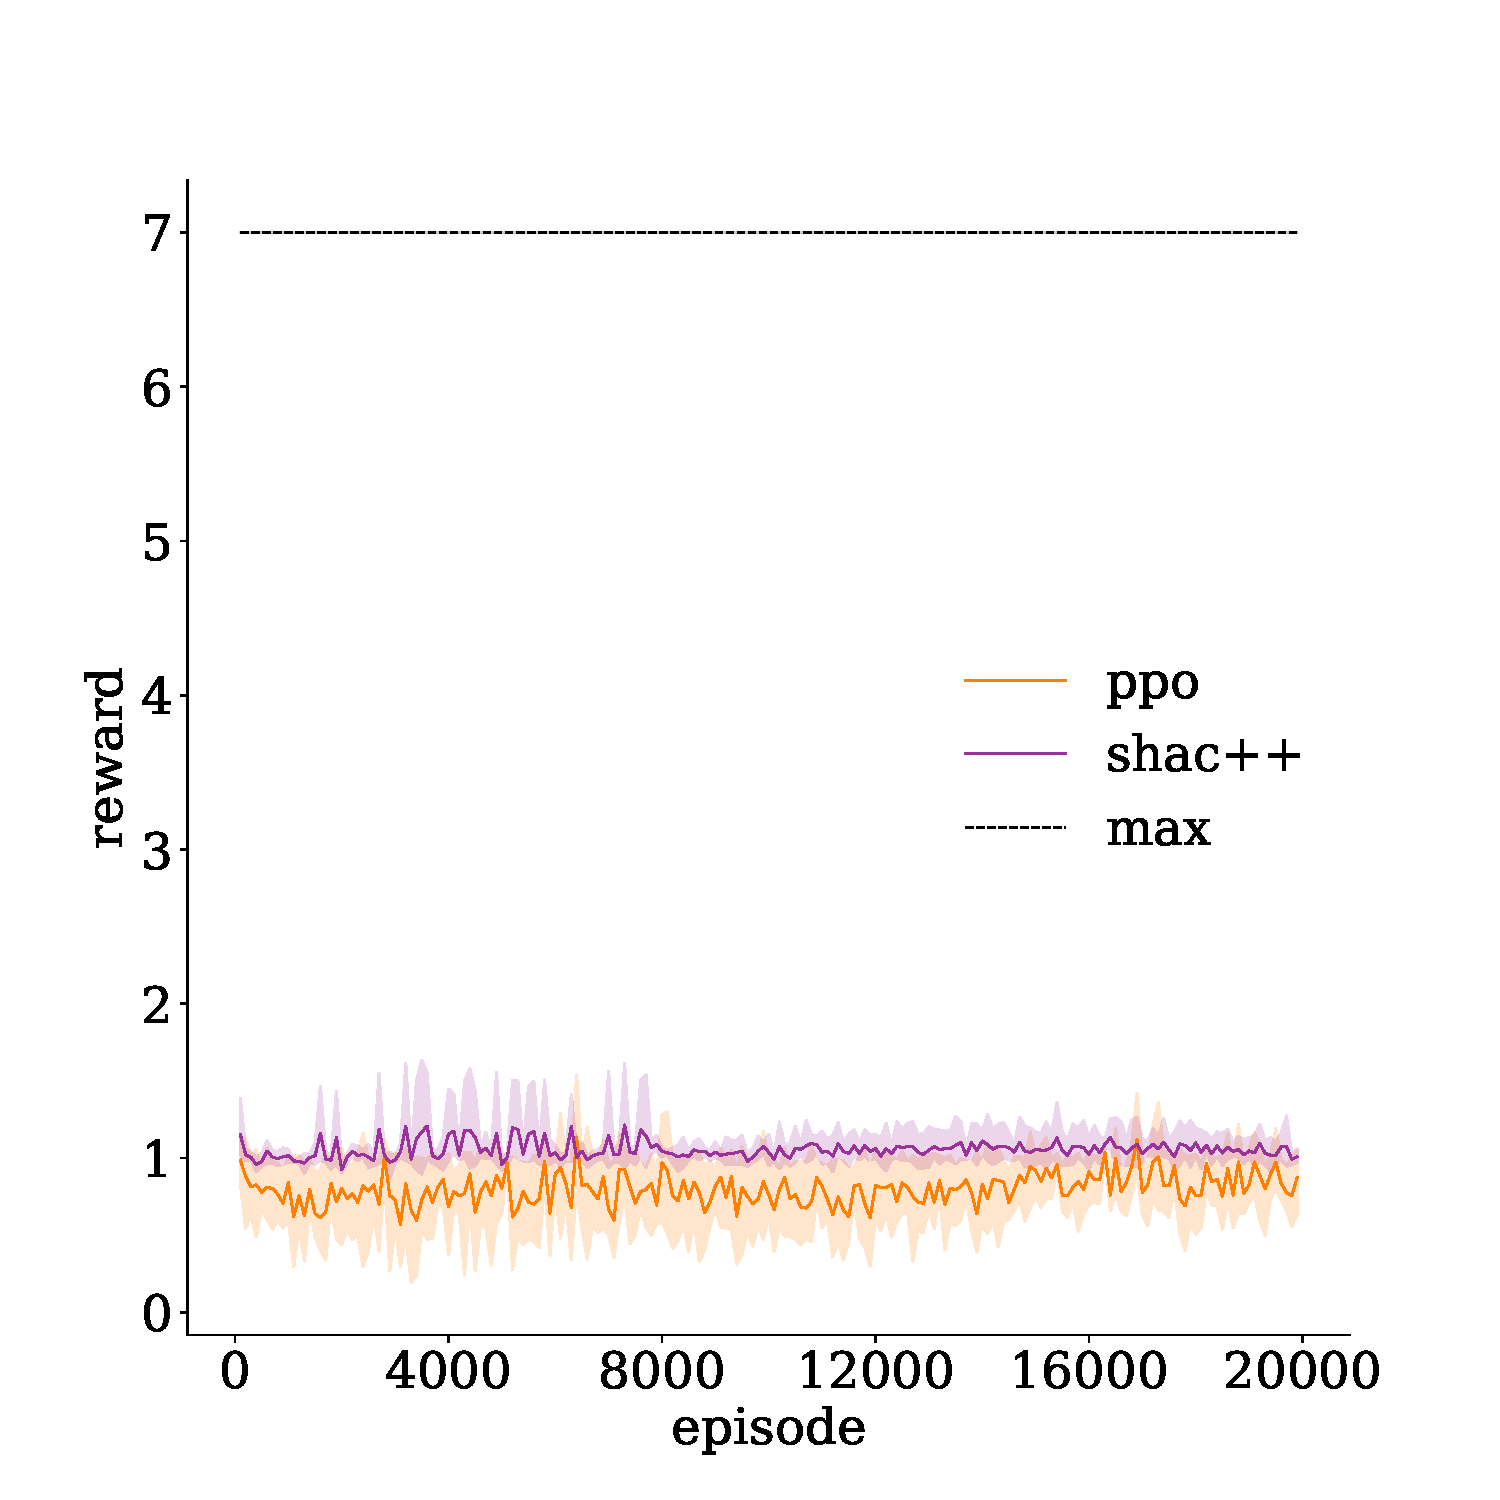
\includegraphics[width=\textwidth]{figs/discovery-1-mlp.pdf}
        \caption{Discovery, MLP, 1 agent}
        \label{apx:fig:discovery-mlp-1}
    \end{subfigure}
    \begin{subfigure}[b]{0.32\textwidth}
        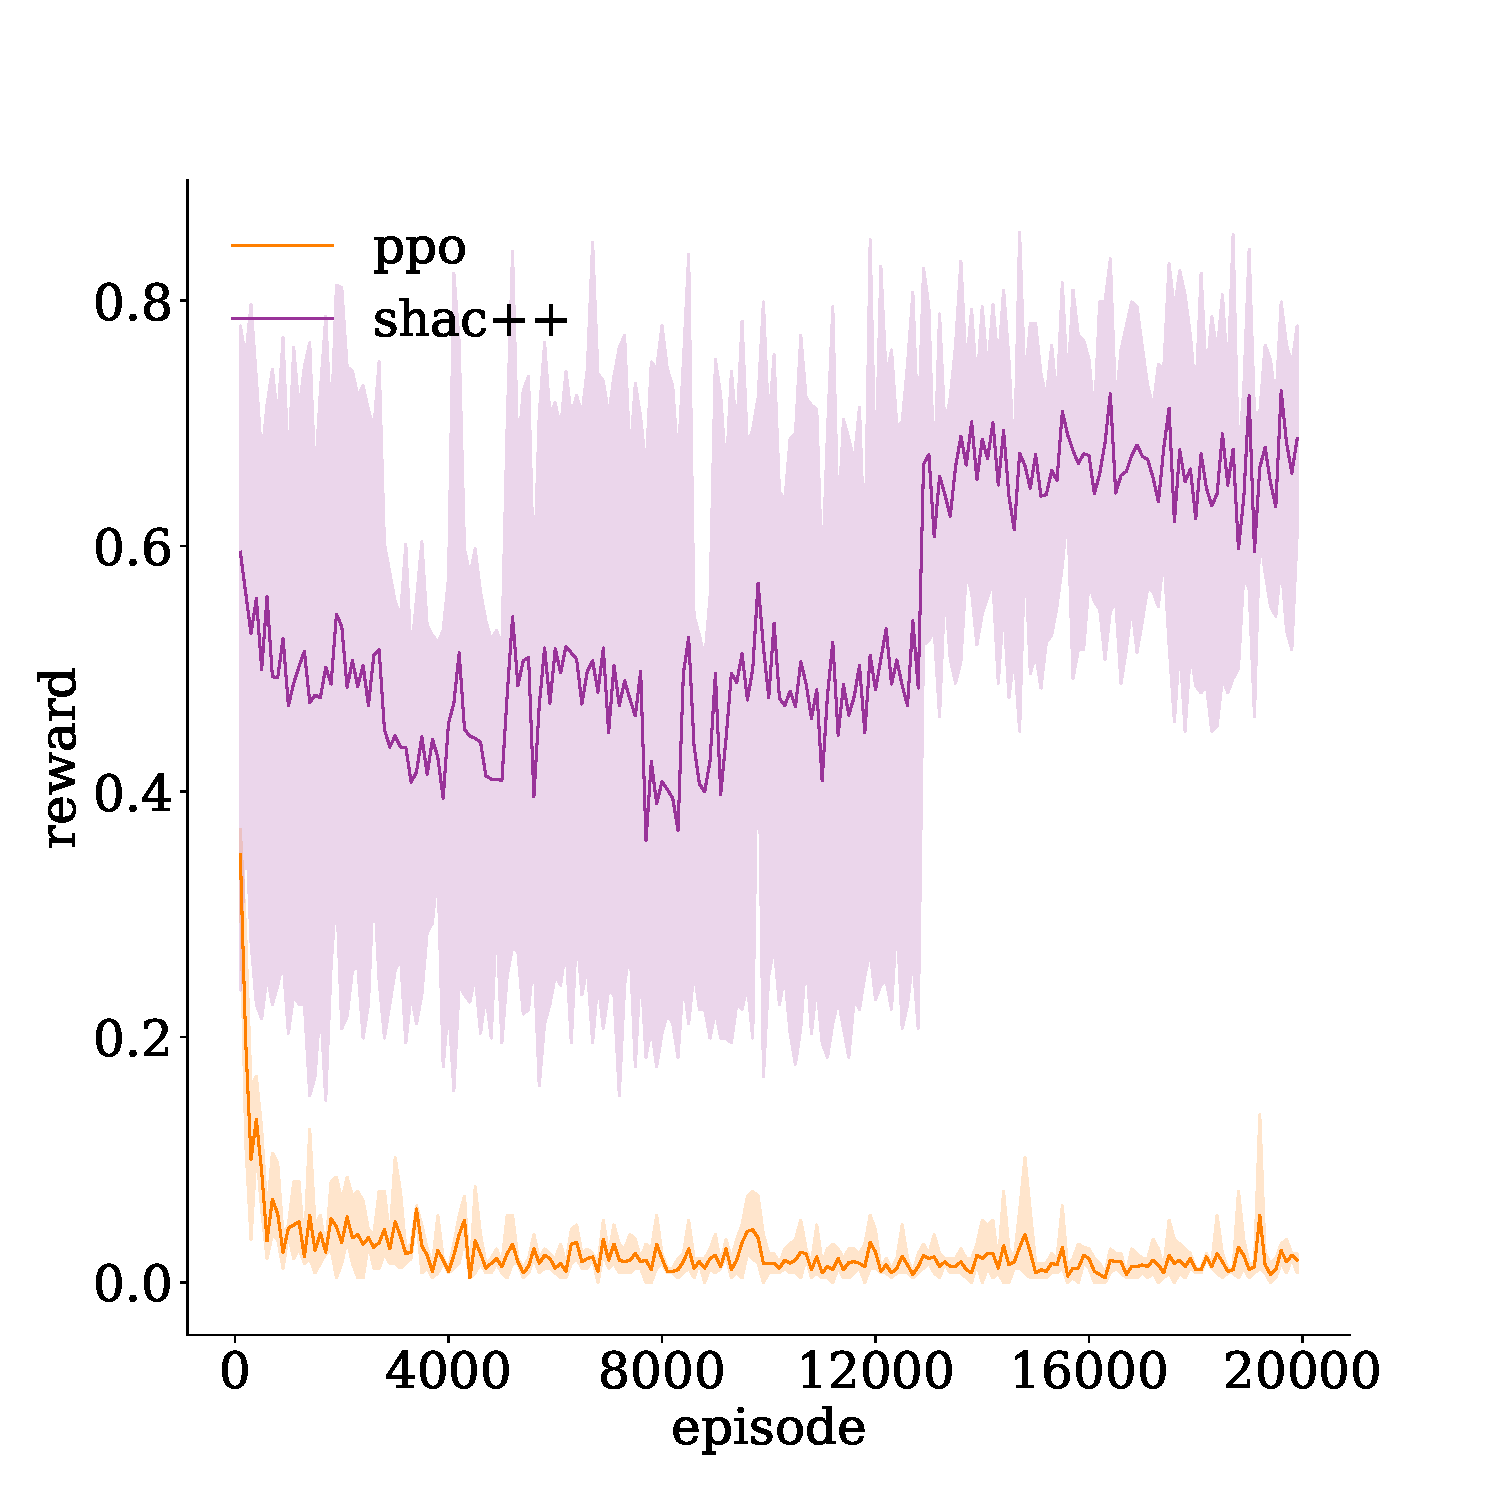
\includegraphics[width=\textwidth]{figs/discovery-3-mlp.pdf}
        \caption{Discovery, MLP, 3 agents}
        \label{apx:fig:discovery-mlp-3}
    \end{subfigure}
    \begin{subfigure}[b]{0.32\textwidth}
        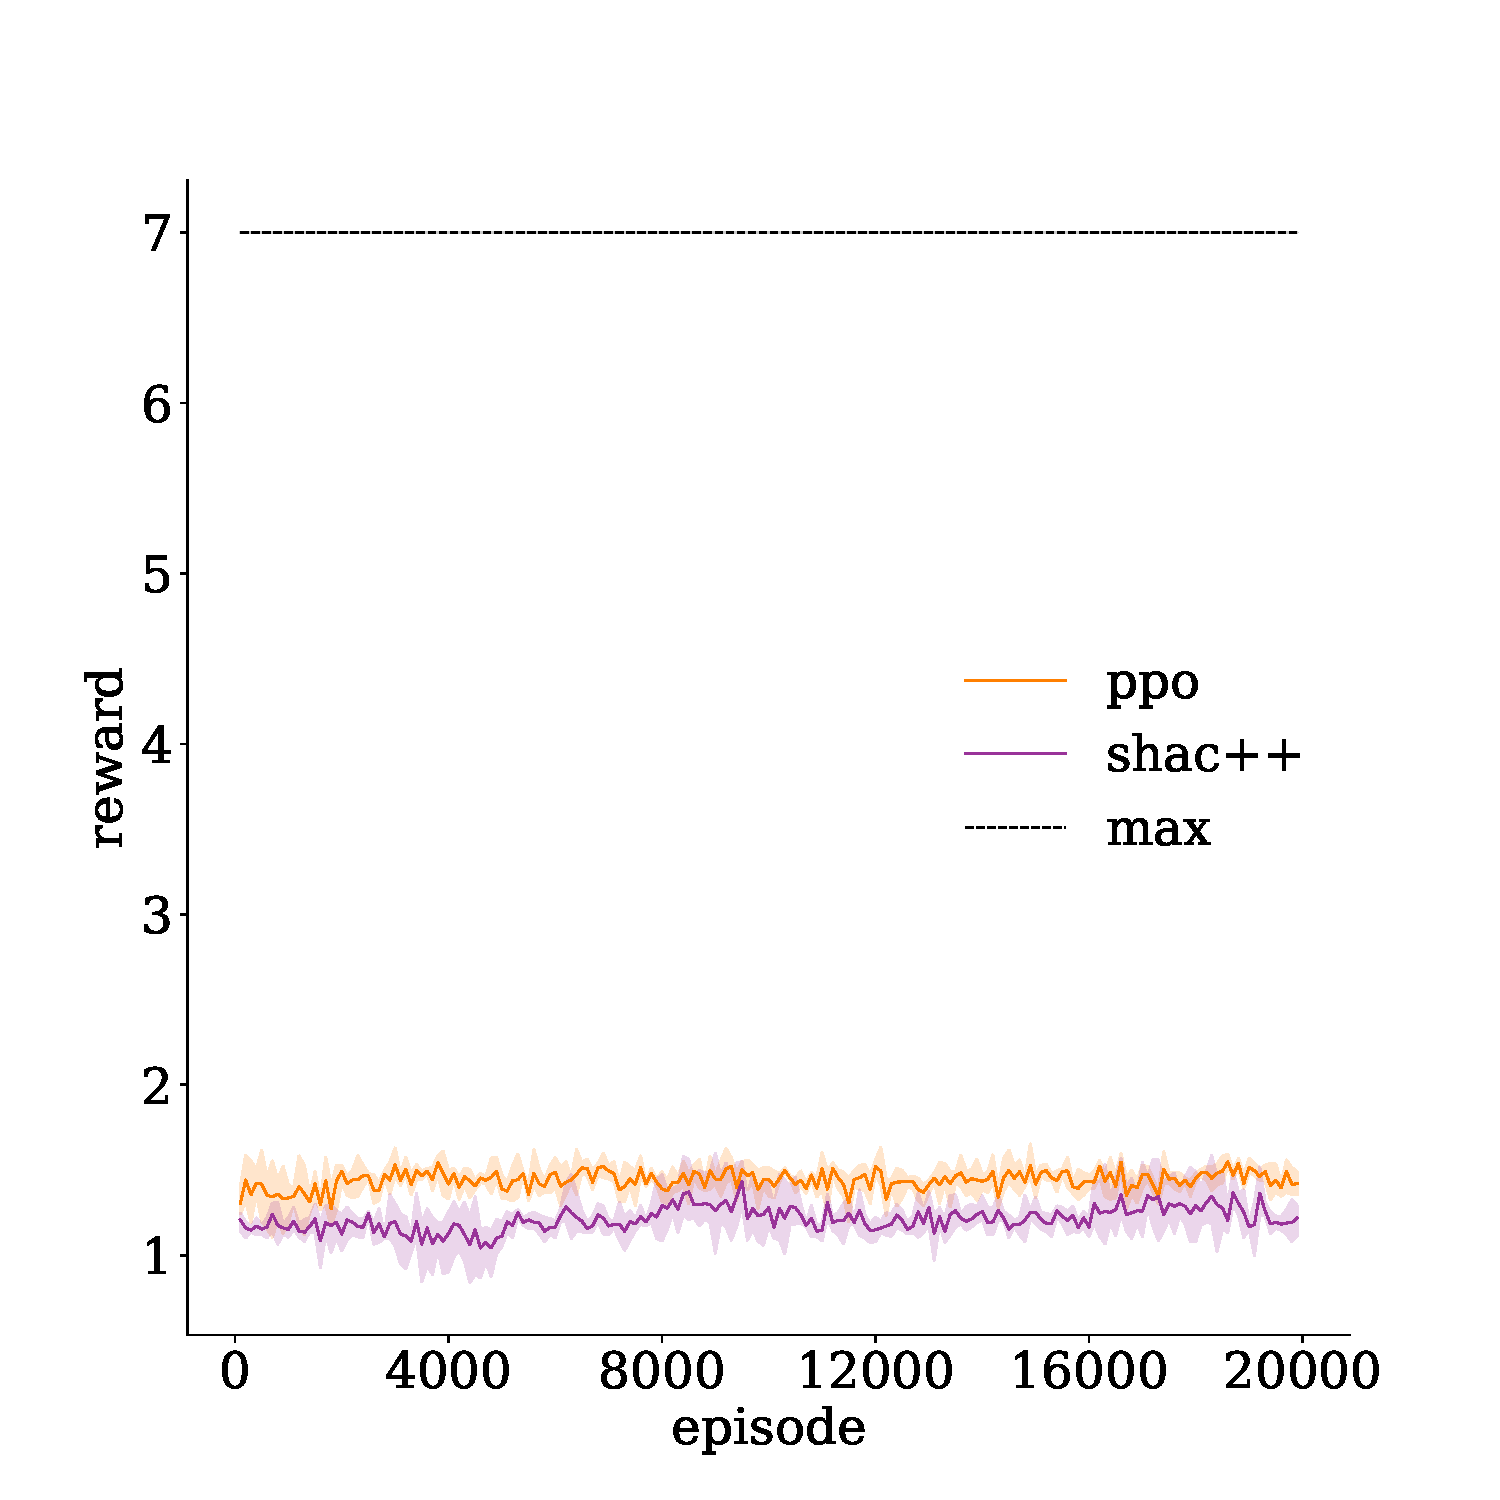
\includegraphics[width=\textwidth]{figs/discovery-5-mlp.pdf}
        \caption{Discovery, MLP, 5 agents}
        \label{apx:fig:discovery-mlp-5}
    \end{subfigure}

    \caption{Comparison between \fname{}, PPO, and SHAC for increasing number of agents for Dispersion, Transport, Discovery, and Sampling scenarios with the MLP architecture.}
    \label{apx:fig:experiments-mlp}

\end{figure}

\begin{figure}[!t]
    \centering
    \begin{subfigure}[b]{0.32\textwidth}
        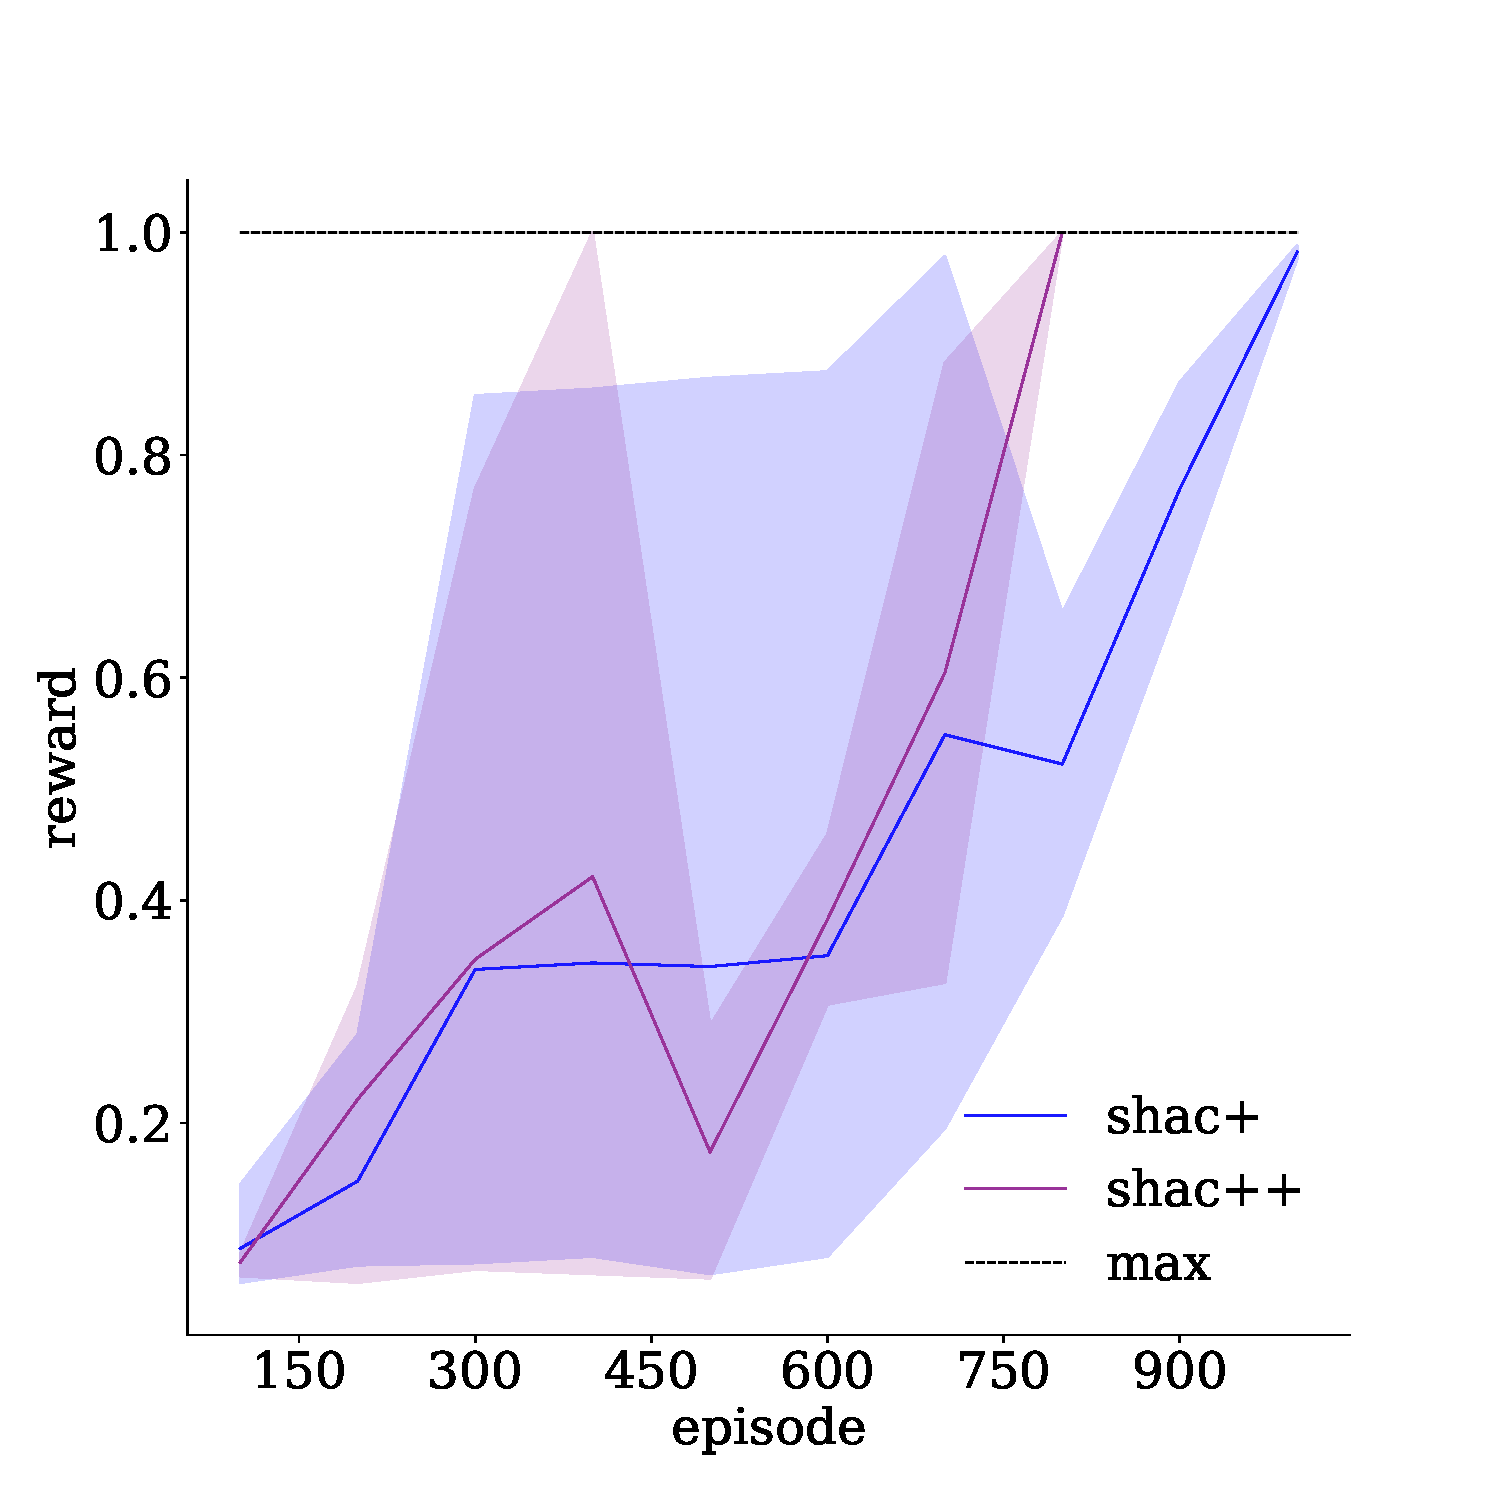
\includegraphics[width=\textwidth]{figs/dispersion-ablation-1-mlp.pdf}
        \caption{Dispersion, MLP, 1 agent}
        \label{fig:dispersion-ablation-mlp-1}
    \end{subfigure}
    \begin{subfigure}[b]{0.32\textwidth}
        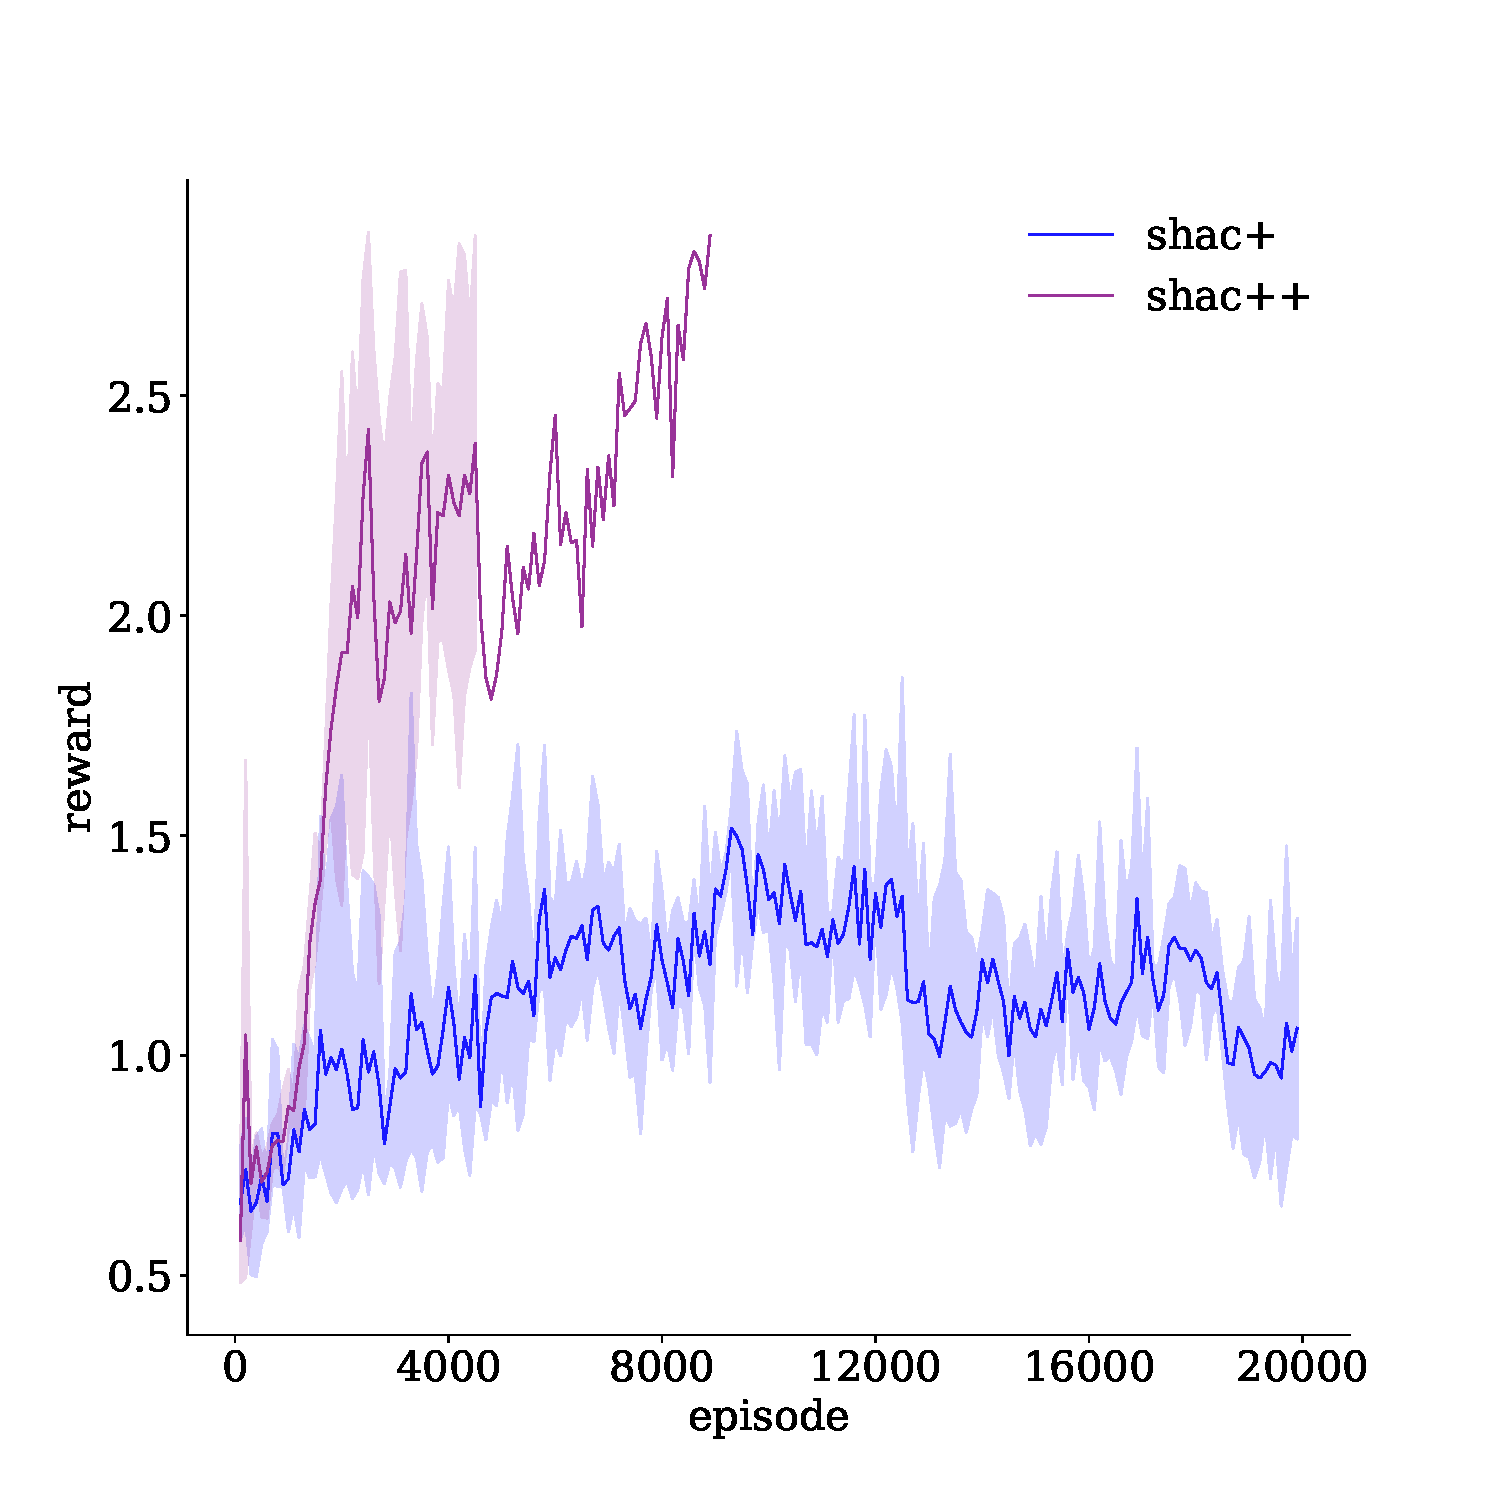
\includegraphics[width=\textwidth]{figs/dispersion-ablation-3-mlp.pdf}
        \caption{Dispersion, MLP, 3 agents}
        \label{fig:dispersion-ablation-mlp-3}
    \end{subfigure}
    \begin{subfigure}[b]{0.32\textwidth}
        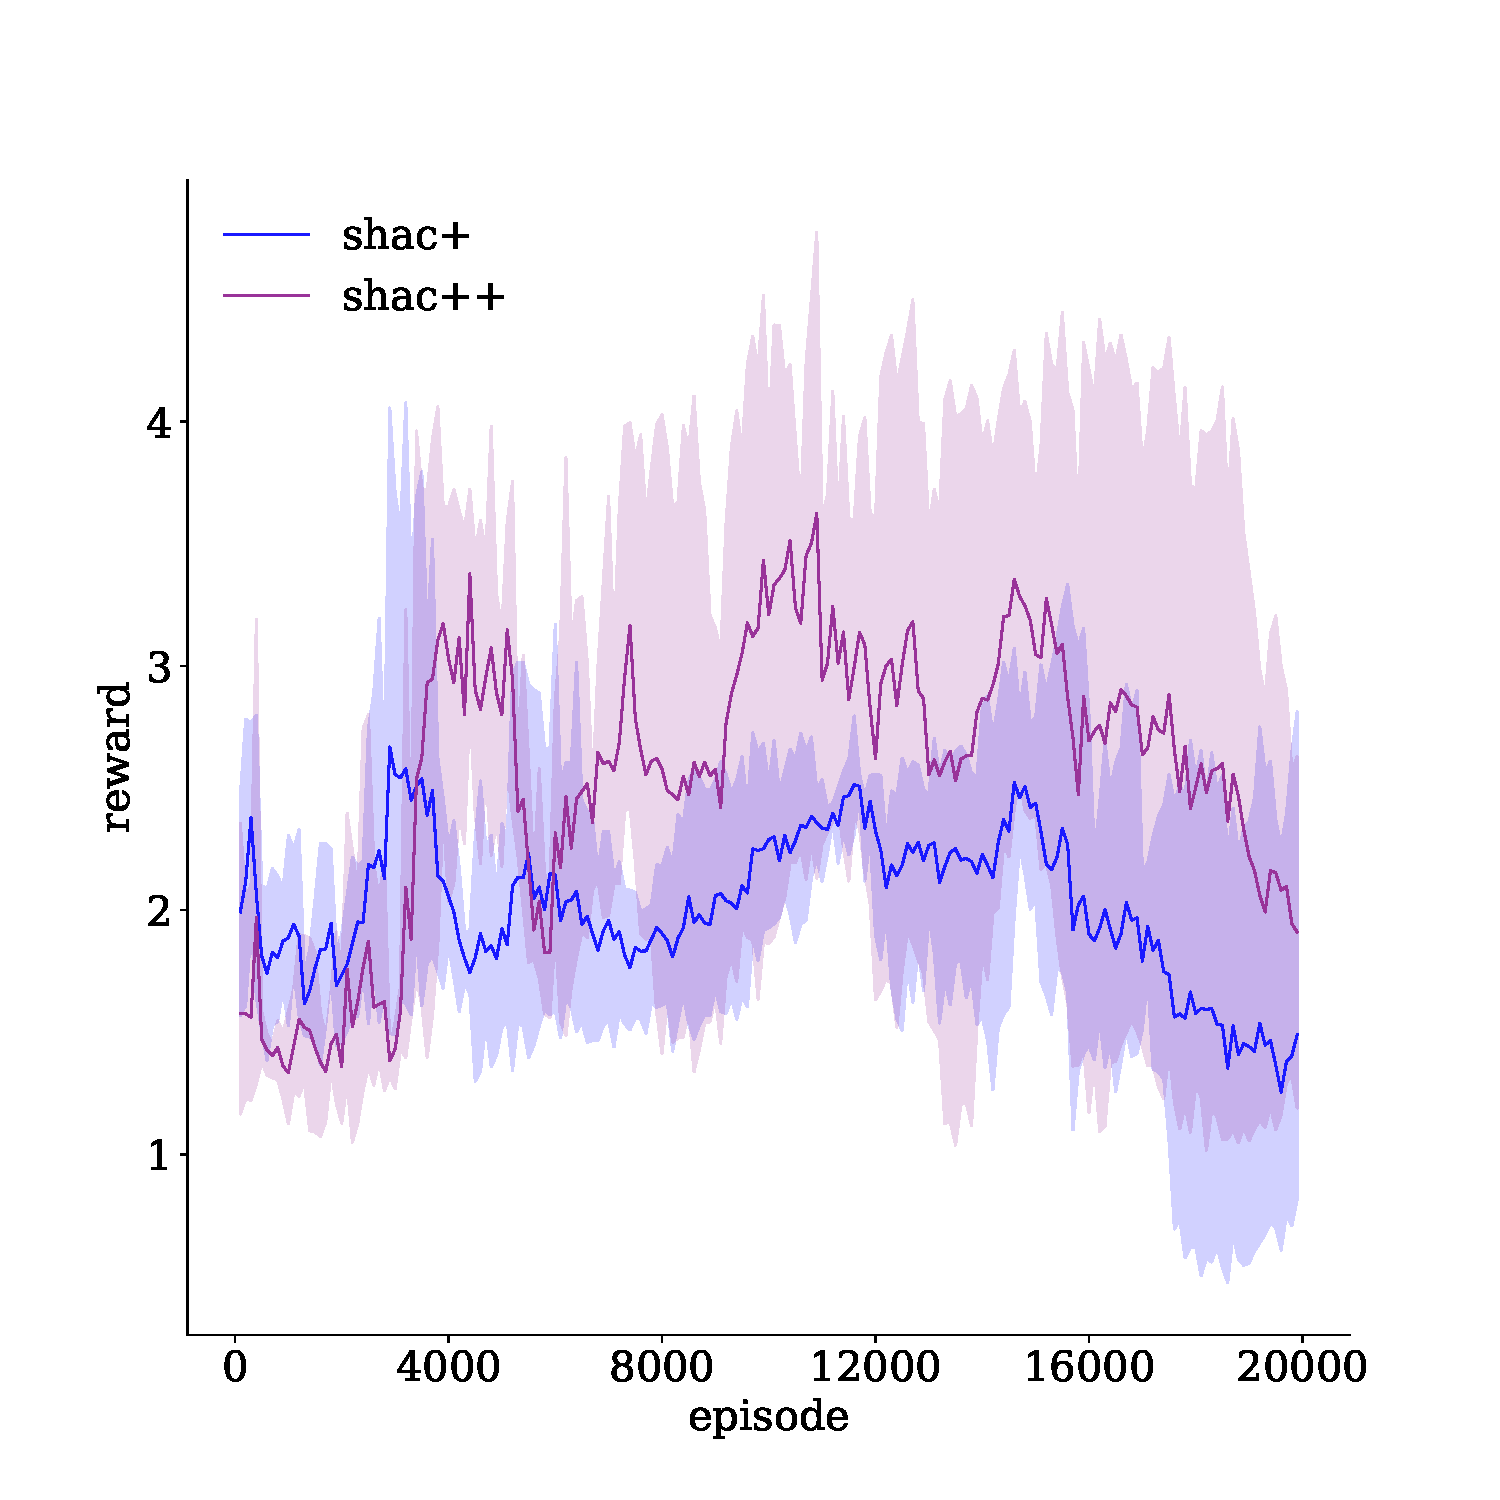
\includegraphics[width=\textwidth]{figs/dispersion-ablation-5-mlp.pdf}
        \caption{Dispersion, MLP, 5 agents}
        \label{fig:dispersion-ablation-mlp-5}
    \end{subfigure}

    \begin{subfigure}[b]{0.32\textwidth}
        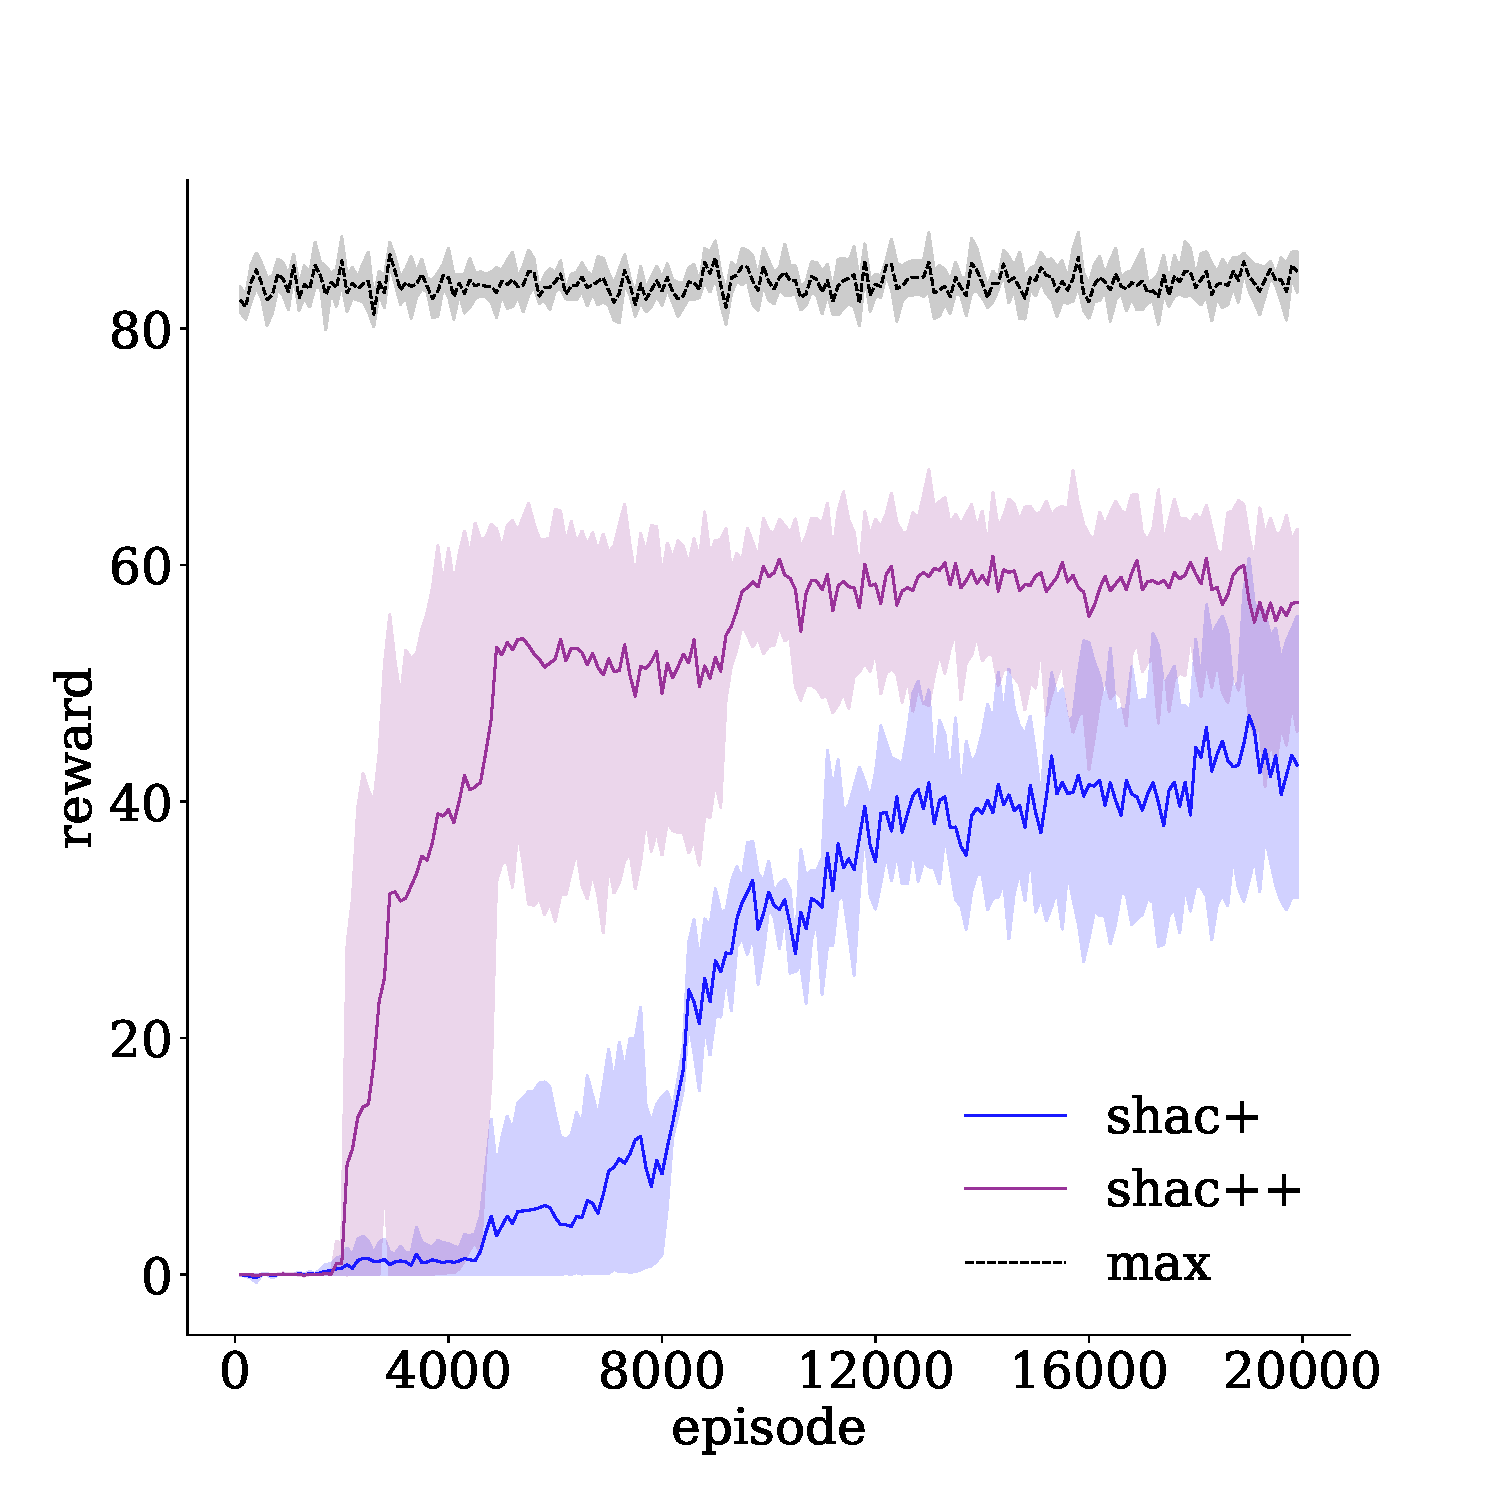
\includegraphics[width=\textwidth]{figs/transport-ablation-1-mlp.pdf}
        \caption{Transport, MLP, 1 agent}
        \label{fig:transport-ablation-mlp-1}
    \end{subfigure}
    \begin{subfigure}[b]{0.32\textwidth}
        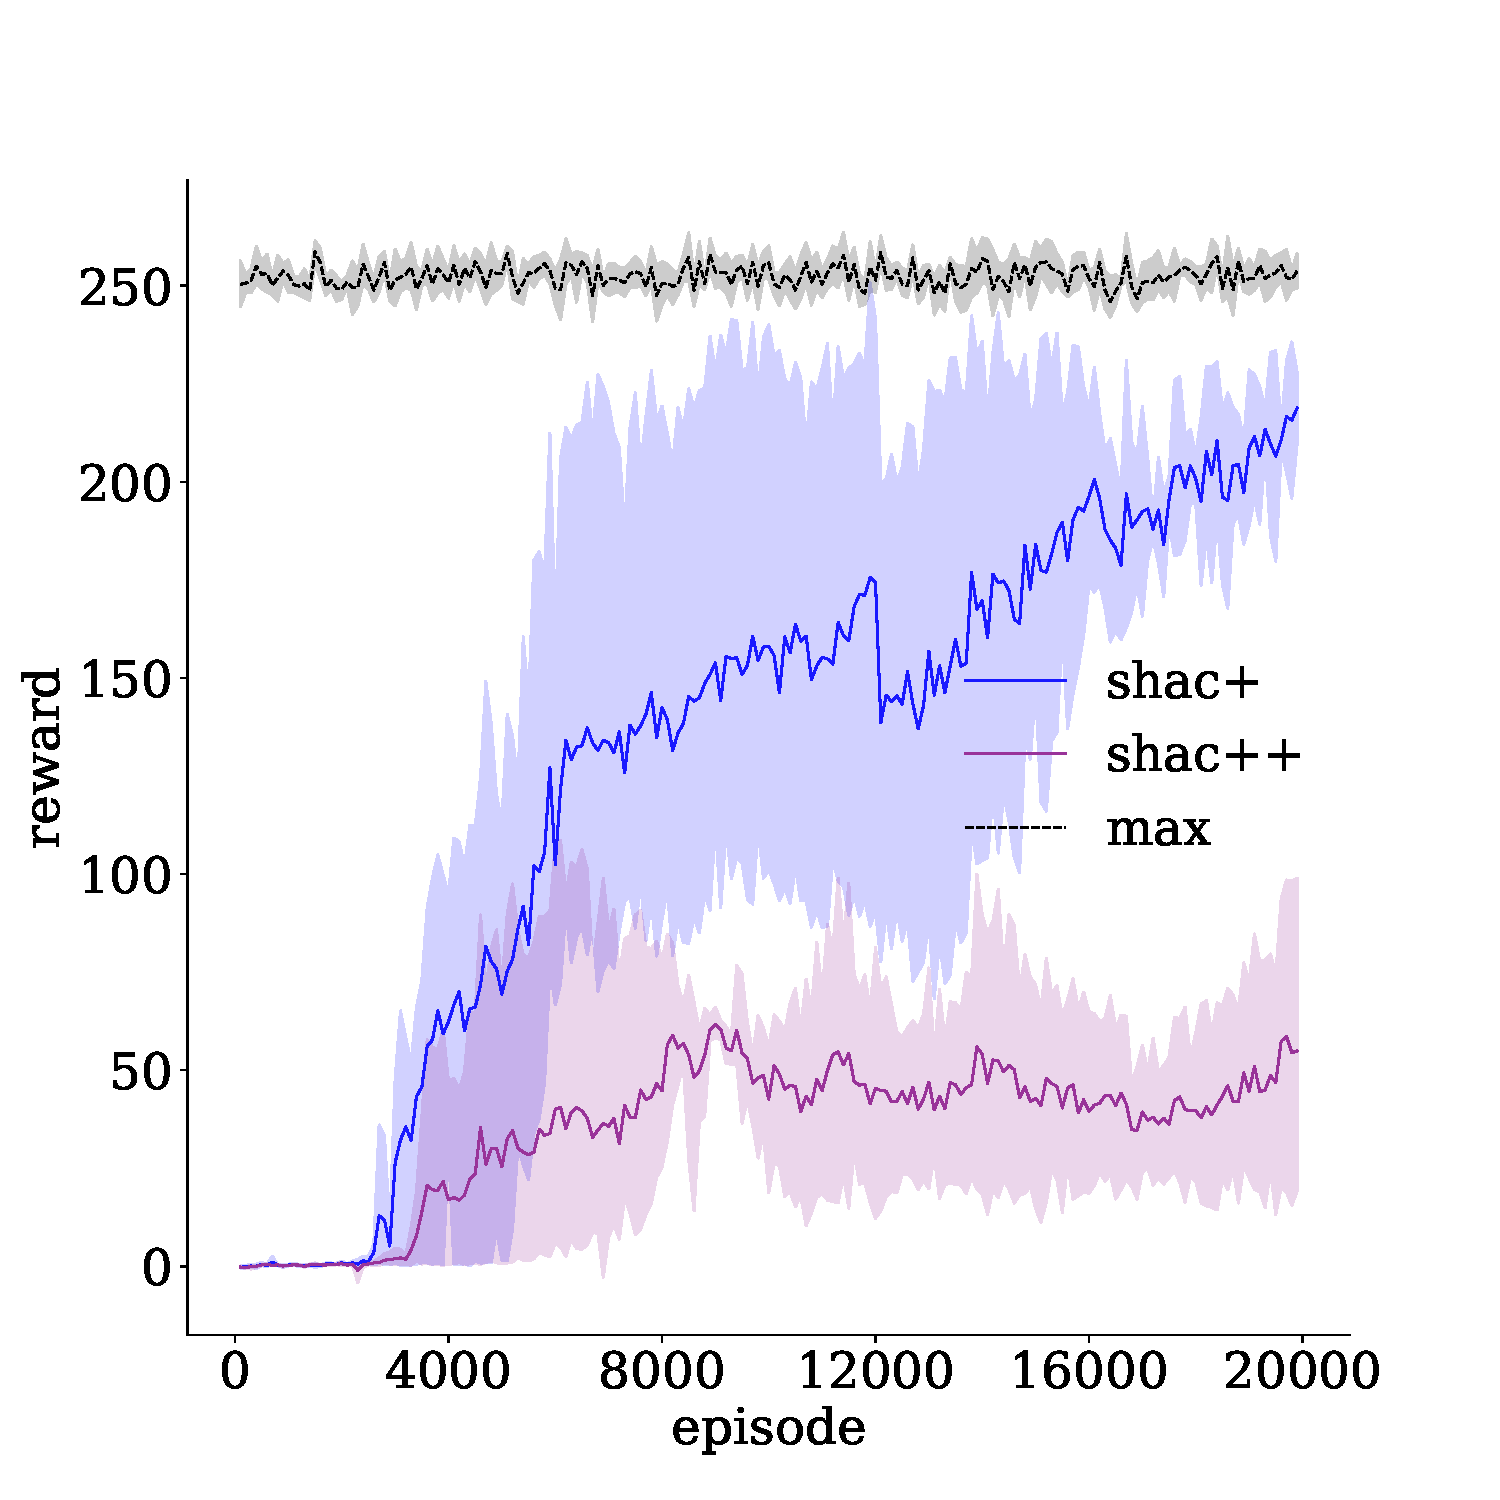
\includegraphics[width=\textwidth]{figs/transport-ablation-3-mlp.pdf}
        \caption{Transport, MLP, 3 agents}
        \label{fig:transport-ablation-mlp-3}
    \end{subfigure}
    \begin{subfigure}[b]{0.32\textwidth}
        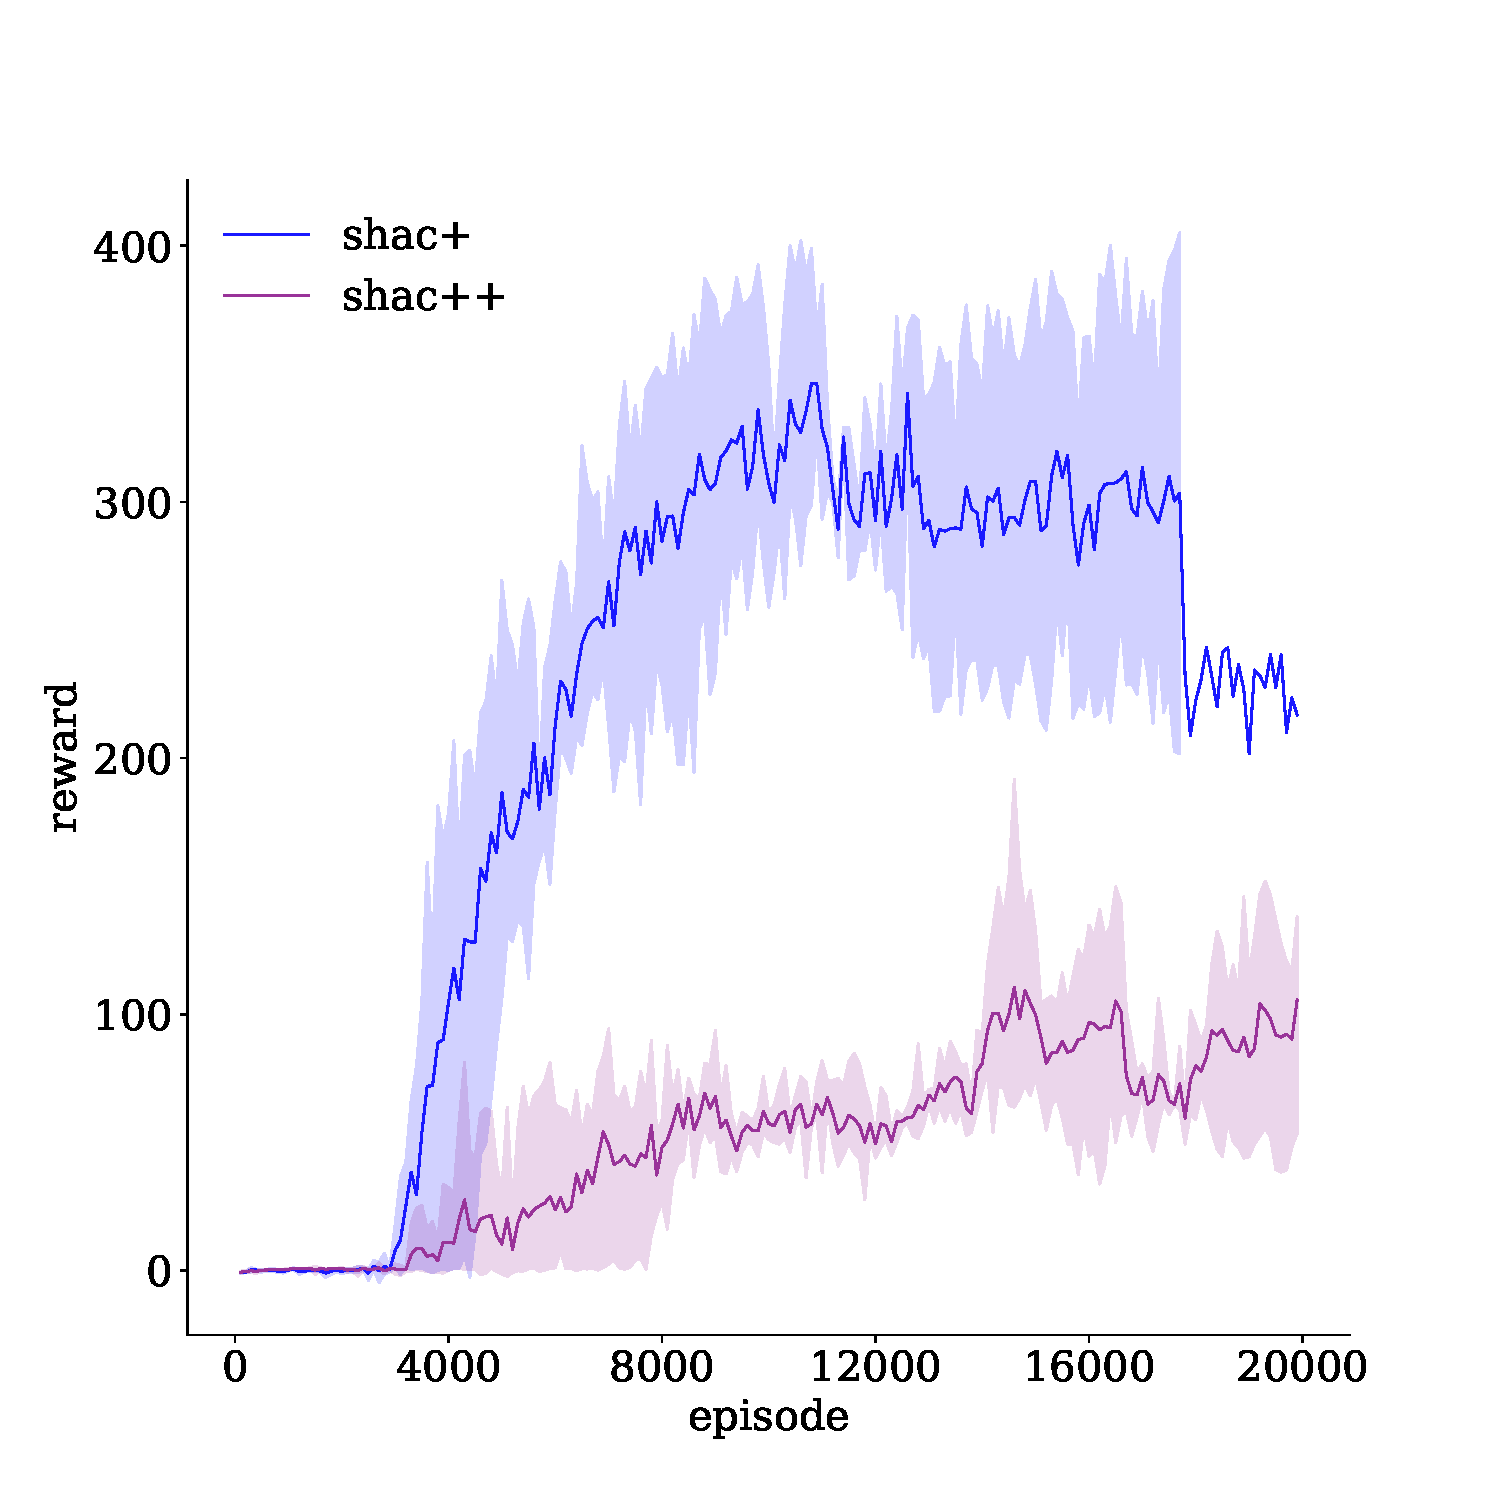
\includegraphics[width=\textwidth]{figs/transport-ablation-5-mlp.pdf}
        \caption{Transport, MLP, 5 agents}
        \label{fig:transport-ablation-mlp-5}
    \end{subfigure}

    \begin{subfigure}[b]{0.32\textwidth}
        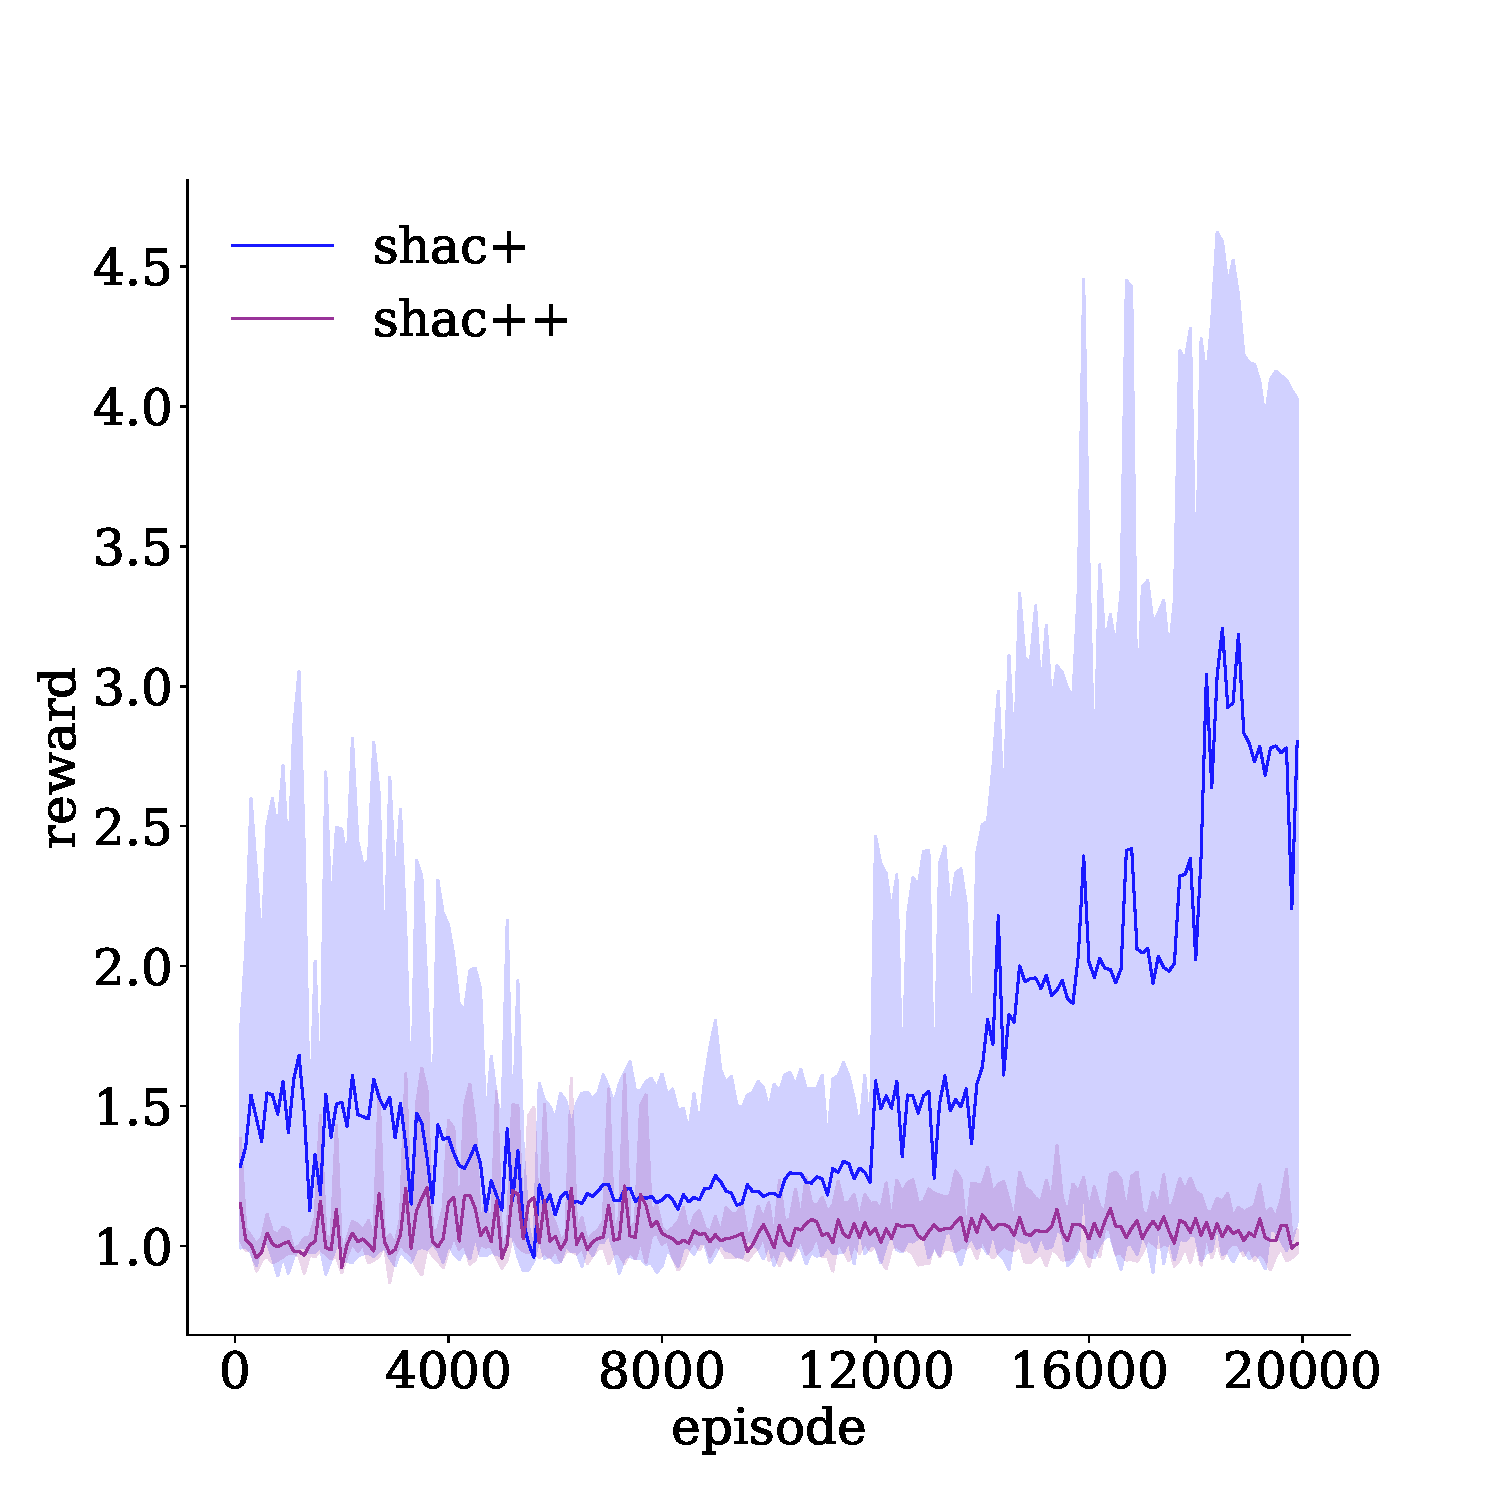
\includegraphics[width=\textwidth]{figs/discovery-ablation-1-mlp.pdf}
        \caption{Discovery, MLP, 1 agent}
        \label{fig:discovery-ablation-mlp-1}
    \end{subfigure}
    \begin{subfigure}[b]{0.32\textwidth}
        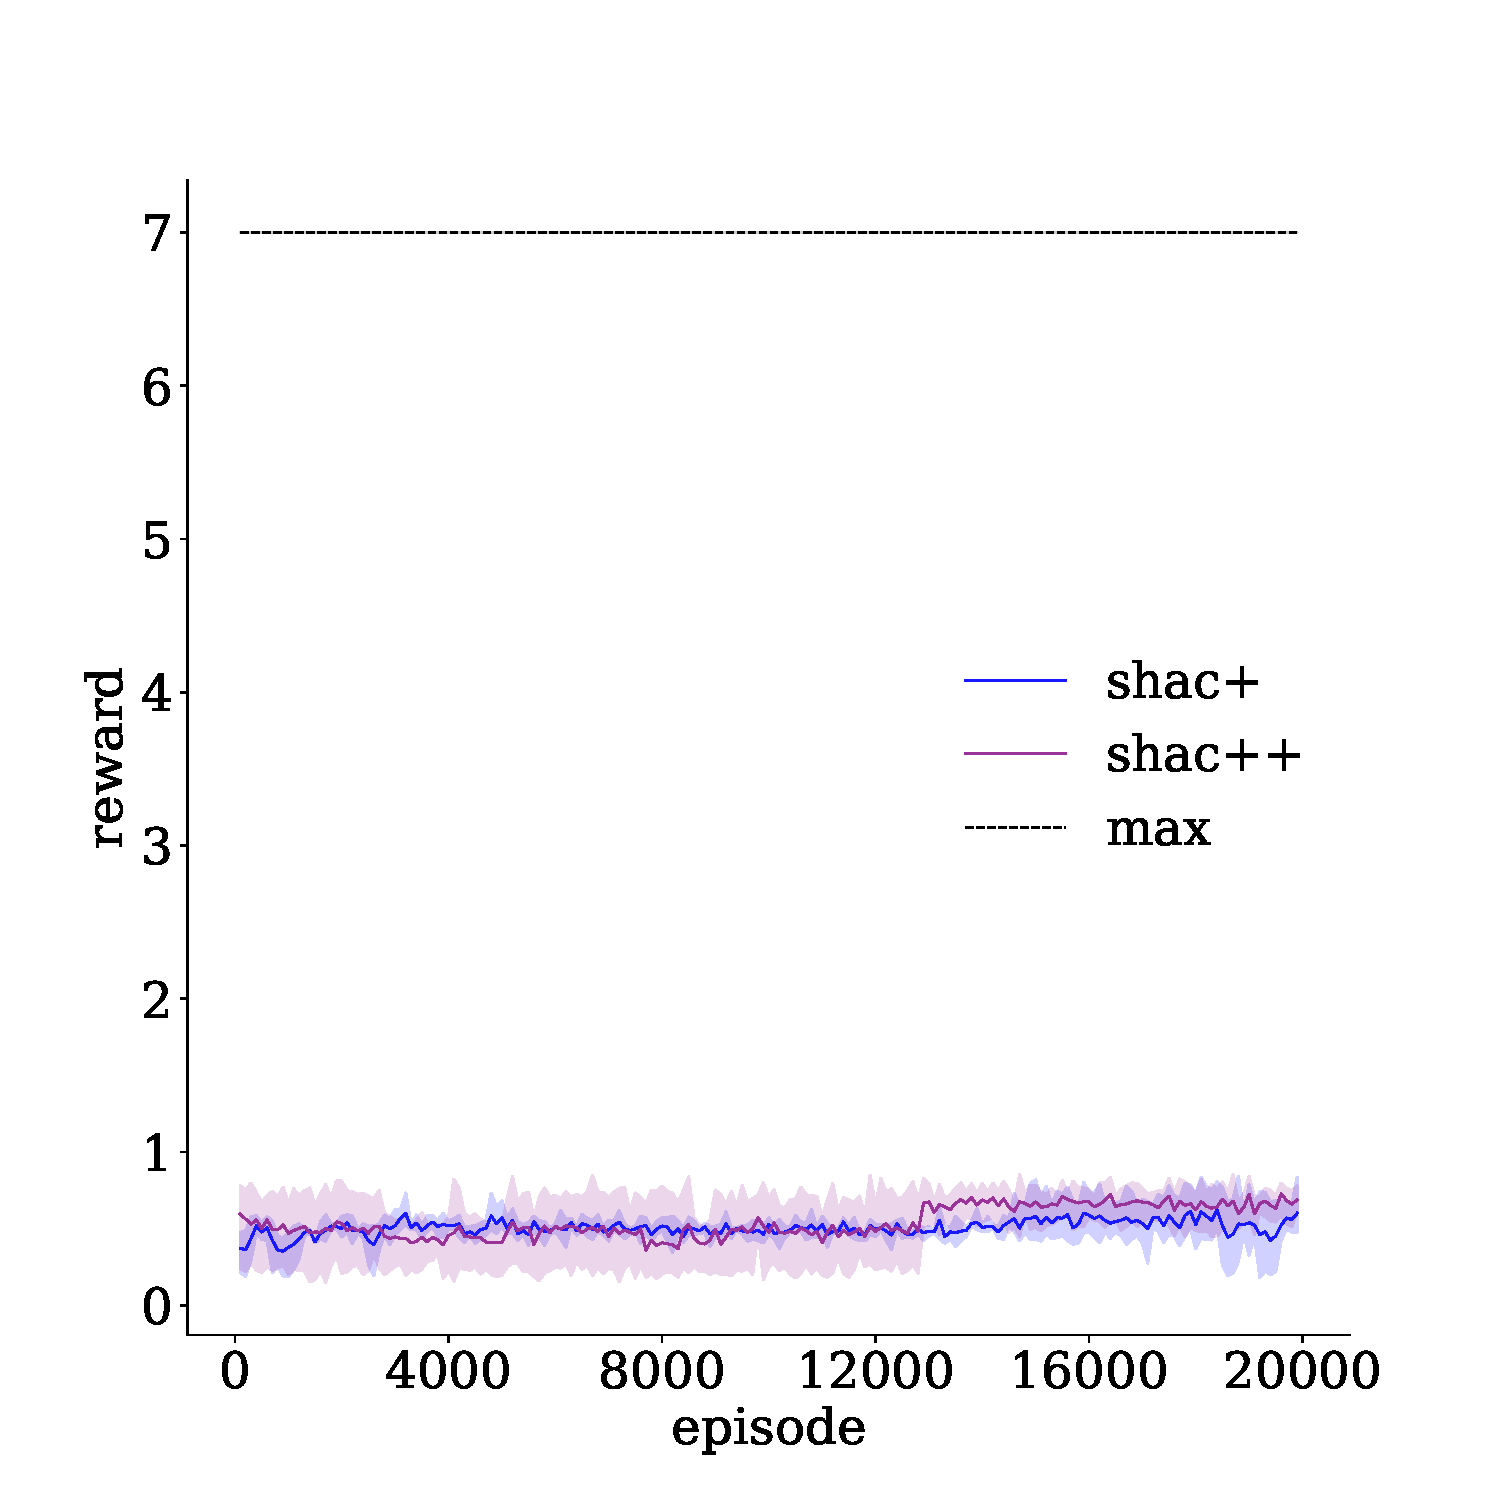
\includegraphics[width=\textwidth]{figs/discovery-ablation-3-mlp.pdf}
        \caption{Discovery, MLP, 3 agents}
        \label{fig:discovery-ablation-mlp-3}
    \end{subfigure}
    \begin{subfigure}[b]{0.32\textwidth}
        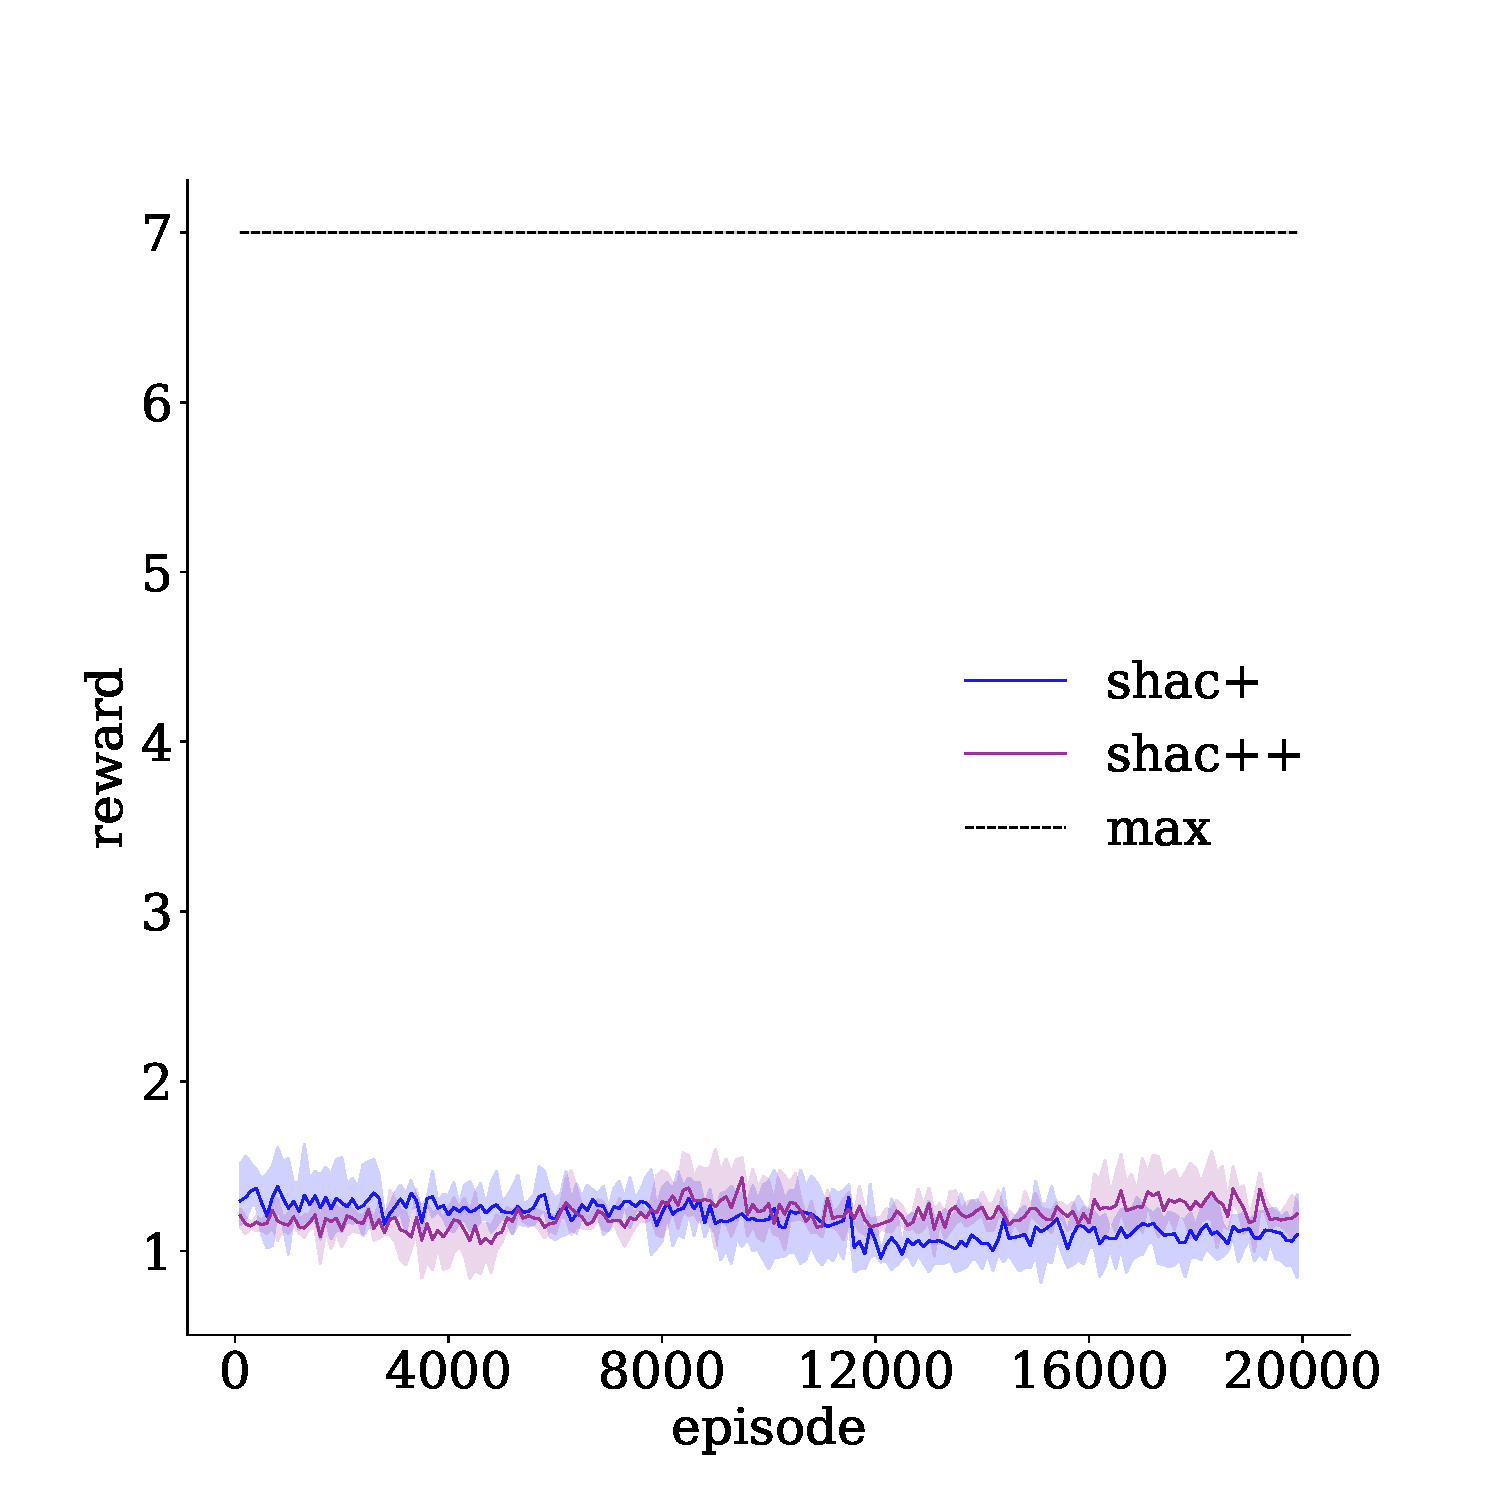
\includegraphics[width=\textwidth]{figs/discovery-ablation-5-mlp.pdf}
        \caption{Discovery, MLP, 5 agents}
        \label{fig:discovery-ablation-mlp-5}
    \end{subfigure}

    \caption{Comparison between \fname{} with and without transition network, labelled \fnamer{}, for increasing number of agents for Dispersion, Transport, Discovery, and Sampling scenarios.}
    \label{fig:ablation}
\end{figure}

\begin{table}[t]
        \centering
        \begin{tabular}{ l l l}
	\toprule
	Parameter & Transformer & MLP \\
	\midrule
	number of training environments & 512 & 512 \\
	training horizon & 32 & 32 \\
	number of evaluation environments & 512 & 512 \\
	evaluation horizon & 512 & 512 \\
	policy layers & 1 & 1 \\
	policy hidden size & 64 & {160, 32, 96} \\
	policy feedforward size & 128 & - \\
	policy heads & 1 & - \\
	policy dropout & 0.1 & 0.1 \\
	policy activation & ReLU & ReLU \\
	policy variance & 1 & 1 \\
	value layers & 1 & 1 \\
	value hidden size & 64 & {160, 32, 96} \\
	value feedforward size & 128 & - \\
	value dropout & 0.0 & 0.0 \\
	value activation & ReLU & ReLU \\
	reward layers & 1 & 1 \\
	reward hidden size & 64 & {160, 32, 96} \\
	reward feedforward size & 128 & - \\
	reward dropout & 0.0 & 0.0 \\
	reward activation & ReLU & ReLU \\
	world layers & 3 & 3 \\
	world hidden size & 64 & 64 \\
	world feedforward size & 128 & 128 \\
	world dropout & 0.0 & 0.0 \\
	world activation & ReLU & ReLU \\
	policy learning rate & 0.001 & 0.001 \\
	reward learning rate & 0.001 & 0.001 \\
	value learning rate & 0.001 & 0.001 \\
	value clip coefficient & None & None \\
	reward clip coefficient & None & None \\
	policy clip coefficient & 1 & 1 \\
	world cache size & 30000 & 30000 \\
	reward cache size & 30000 & 30000 \\
	value cache size & 30000 & 30000 \\
	world/value/reward batch size & 1000 & 1000 \\
	world/value/reward cooldown epochs & 10 & 10 \\
	world cache bins & 25 & 25 \\
	reward cache bins & 9 & 9 \\
	value cache bins & 9 & 9 \\
	$\alpha$ & 1.0 & 1.0 \\
	early stopping - max reward fraction & 0.9 & 0.9 \\
	early stopping - max envs fraction & 0.9 & 0.9 \\
	seed & {42, 43, 44} & {42, 43, 44} \\
	max episodes & 20000 & 20000 \\
	epochs between environment resets & 10 & 10 \\
	epochs between evaluations & 100 & 100 \\
	$\gamma$ & 0.99 & 0.99 \\
	$\lambda$ & 0.95 & 0.95 \\
	\bottomrule
\end{tabular}

        \caption{SHAC/\fname{}/\fnamer{} Hyperparameters}
        \label{apx:tab:shac}
\end{table}

\begin{table}[t]
        \centering
        \begin{tabular}{ l l l}
	\toprule
	Parameter & Transformer & MLP \\
	\midrule
	number of training environments & 512 & 512 \\
	training horizon & 32 & 32 \\
	number of evaluation environments & 512 & 512 \\
	evaluation horizon & 512 & 512 \\
	policy layers & 1 & 1 \\
	policy hidden size & 64 & {160, 32, 96} \\
	policy feedforward size & 128 & - \\
	policy heads & 1 & - \\
	policy dropout & 0.1 & 0.1 \\
	policy activation & ReLU & ReLU \\
	policy variance & 1 & 1 \\
	value layers & 1 & 1 \\
	value hidden size & 64 & {160, 32, 96} \\
	value feedforward size & 128 & - \\
	value dropout & 0.0 & 0.0 \\
	value activation & ReLU & ReLU \\
	policy learning rate & 0.001 & 0.001 \\
	value learning rate & 0.001 & 0.001 \\
	early stopping - max reward fraction & 0.9 & 0.9 \\
	early stopping - max envs fraction & 0.9 & 0.9 \\
	seed & {42, 43, 44} & {42, 43, 44} \\
	max episodes & 20000 & 20000 \\
	epochs between environment resets & 10 & 10 \\
	epochs between evaluations & 100 & 100 \\
	$\gamma$ & 0.99 & 0.99 \\
	$\lambda$ & 0.95 & 0.95 \\
	$\alpha$ & 1.0 & 1.0 \\
	\bottomrule
\end{tabular}

        \caption{PPO Hyperparmeters}
        \label{apx:tab:ppo}
\end{table}

